\documentclass[a4paper,12pt,oneside]{book}
\usepackage{stata}
\usepackage{graphicx}
\usepackage{longtable}
\setlength{\parskip}{1em}
\setlength{\parindent}{0pt}
\renewcommand{\baselinestretch}{1.5}
\begin{document}
\begin{titlepage}
    \begin{center}
        \vspace*{1cm}
 
        \Huge
        \textbf{Logistic Regression using Stata}
 
        \vspace{0.5cm}
        \LARGE
        Theory and Application
 
        \vspace{1.5cm}
 
        \textbf{Najib A. Mozahem}
 
        \vfill
 
        \vspace{0.8cm}
 
    \end{center}
\end{titlepage}
\tableofcontents
\chapter{Logistic Regression - The Theory}
\section{Contingency Tables}
\subsection{Two-by-Two Tables}
When the outcome that we are interested in can take on one of two values, the variable is referred to as a binary variable. As an example, consider the data shown in Table ~\ref{table:first}. The table shows the records for 31 
students, where the first column indicates whether the student has withdraw from or completed a certain course, while the second column shows the major of the student. In this case, the outcome of interest is 
whether the student completed the course or whether he/she withdrew from the course. These are the only two possible outcomes. Hence, the variable is binary. The other variable is also binary since it also has two 
possible values: engineering and business. 
\begin{longtable}[c]{ c c }
	\caption{Records of students.\label{table:first}}\\
		\hline
		\bf Outcome & \bf College \\
		\hline
		Withdraw & Engineering \\
		Withdraw & Engineering \\
		Finish & Business \\
		Finish & Business \\
		Finish & Business \\
		Finish & Engineering \\
		Finish & Engineering \\
		Finish & Engineering \\
		Withdraw & Engineering \\
		Finish & Business \\
		Withdraw & Engineering \\
		Finish & Business \\
		Withdraw & Engineering \\
		Withdraw & Engineering \\
		Finish & Business \\
		Finish & Business \\
		Withdraw & Business \\
		Withdraw & Business \\
		Withdraw & Business \\
		Finish & Business \\
		Finish & Engineering \\
		Withdraw & Engineering \\
		Finish & Business \\
		Finish & Business \\
		Finish & Engineering \\
		Withdraw & Business \\
		Withdraw & Engineering \\
		Withdraw & Engineering \\
		Finish & Engineering \\
		Finish & Business \\
		Finish & Business \\
	\hline
\end{longtable}
The question that we would like to ask is whether students from both colleges are equally likely to withdraw from the course. To find the answer, we create a two-by-two table. 
The table is shown in Table ~\ref{table:countfirst}. This table sums up the results. We see that there is a total of 16 business students, four of whom withdrew from the course. We also see that there is a total of 15 engineering students, 
nine of whom withdrew from the course. This means that a proportion of 4/16 = 0.25 of business students withdrew from the course, compared to a proportion of 9/15 = 0.6 of engineering students. If an engineering student 
enrolls in the course, we calculate that the probability that he or she will withdraw from the course is 0.6. If a business student enrolled in the course, we calculate that the probability that he or she will withdraw 
from the course is 0.25. Therefore, we see that engineering students are more likely to withdraw from the course than business students.
\begin{table}[h!t]
	\caption{Cross classification of college and outcome.} \label{table:countfirst}
	\centering
	\begin{tabular}{c |c c| c}
	\hline
	{} & \multicolumn{2}{|c|}{Outcome} & {} \\
	\hline
	\bf College & \bf Withdraw & \bf Finish & \bf Total \\
	Business & 4 & 12 & 16 \\
	Engineering & 9 & 6 & 15 \\
	\hline
	\end{tabular}
\end{table}
\subsection{The Odds Ratio}
In order to better compare the two groups, we can use the concept of \textbf{odds ratios}. To do that, we need to calculate the odds that a student will withdraw from the course. This can be done using the equation:

$$ odds=\frac{Probability\, of\, withdrawal}{1-(probability\, of\, withdrawal)} $$

The odds of withdrawal for an engineering student is 0.6/(1-0.6) = 1.5. The odds of withdrawal for a business student is 0.25/(1-0.25) = 0.33. 

The odds are never negative. They are zero or greater than zero. When the odds are equal to one, this means that the probability of both outcomes are equal (0.5/(1-0.5) = 1). In the case of engineering students, 
since the odds of withdrawal are 1.5, this means that the probability of withdrawal is 1.5 times the probability of finishing the course. For business students, the probability of withdrawal is 0.33 times the 
probability of finishing the course.

Now that we have the odds for each row in Table ~\ref{table:countfirst}, we can calculate the odds ratio:

$$ odds\, ratio = \frac{odds_{engineering}}{odds_{business}}=\frac{1.5}{0.33}=4.5 $$

Since the odds cannot be negative, the odds ratio cannot be negative as well. When the odds of an event are equal in both rows (Table ~\ref{table:countfirst}), the odds ratio will be equal to one. When the odds of the numerator is greater 
than the odds of the denominator, the odds ratio will be greater than one. This means that the probability of the event is higher in the row that is associated with the numerator. In our case, the odds ratio is 4.5, 
which is larger than one. This means that the probability of the event, which is withdrawal in our case, is higher in the numerator, which is engineering students in our case. This means that engineering students are more likely to withdraw 
from the course than business students. If, on the other hand, the odds ratio is less than one, then this means that the probability of the event in the denominator are higher.

As you can see, the odds ratio allows us to compare the incidence of an event between groups. If the event is equally probable in both groups, then the odds ratio will be one. In such a case, we say that 
the event (withdrawal in our case) and the group (college in our case) are independent. This means that withdrawal does not depend on college.
\subsection{Two-by-Three Tables}
The above logic remains intact when instead of a binary variable such as college, we have a variable that divides students into the groups sophomore, junior, and senior. In this case, the outcome variable is binary, 
but the other variable is not, since it divides the students into more than two groups.

As an example, consider the data shown in Table ~\ref{table:countcatmore}. The odds of withdrawal for sophomores, junior, and senior students are:

$$ odds_{sophomore}=\frac{12/32}{1-\frac{12}{32}}=0.6 $$

$$ odds_{junior}=\frac{6/36}{1-\frac{6}{36}}=0.2 $$

$$ odds_{senior}=\frac{5/30}{1-\frac{5}{30}}=0.2 $$

Since the odds for all groups are less than one, then the probability of course withdrawal is less than the probability of finishing the course in each of them. We can also compute the odds ratios in order to compare 
the odds of each group:

$$ \frac{odds_{sophomore}}{odds_{junior}}=\frac{0.6}{0.2}=3 $$

$$ \frac{odds_{sophomore}}{odds_{senior}}=\frac{0.6}{0.2}=3 $$

$$ \frac{odds_{junior}}{odds_{senior}}=\frac{0.2}{0.2}=1 $$

The results indicate that the probability of withdrawal are highest in sophomore students.
\begin{table}[h!t]
	\caption{Cross classification of standing and outcome.} \label{table:countcatmore}
	\centering
	\begin{tabular}{c |c c| c}
	\hline
	{} & \multicolumn{2}{|c|}{Outcome} & {} \\
	\hline
	\bf Standing & \bf Withdraw & \bf Finish & \bf Total \\
	Sophomore & 12 & 20 & 32 \\
	Junior & 6 & 30 & 36 \\
	Senior & 5 & 25 & 30 \\
	\hline
	\end{tabular}
\end{table}
The above exercise is useful when we want to compare the probabilities of an event across certain groups. We saw that the probability of withdrawal is affected by the major of the student. 
In the second example, we saw that the probability of withdrawal was affected by whether the student was a sophomore, junior, or senior.

This type of analysis however will not take us very far. The reason is that usually, we are interested in studying the effect that several variables have on the outcome. What if we wanted to see 
whether the withdrawal rate was affected by the major, standing, and GPA, all at the same time? In this case, we need to use the statistical technique of logistic regression. 
\section{Logistic Regression}
We will start by considering the simplest case in which there is a single independent variable. In linear regression, the model is represented by the linear equation:

$$ y=ax+b $$

In the above equation, y is the dependent variable, x is the independent variable, a is the slope, and b is the y-intercept. One of the nice things about linear regression is how easy it is to interpret 
the relationship between the dependent variable and the independent variable. As an example, assume that we have the following linear equation:

$$y=3x+2$$

If x is equal to 2, y will be equal to 8, and if x is equal to 3, y will be equal to 11. Note that for every one unit increase in x, the value of y increases by 3, which is the value of the slope. 
This is the definition of the slope. It is the amount by which the dependent variable changes when the independent variable increases by one. The slope is important for two reasons. The first reason 
relates to the sign. If the slope is positive, then any increase in the independent variable will lead to an increase in the dependent variable. The more I eat, the heavier I get. If the slope is negative, 
then an increase in the independent variable will lead to a decrease in the dependent variable. The more I buy food, the less money I have.

The second reason relates to the magnitude of the slope. The larger the magnitude of the slope, the greater the effect that the independent variable has on the dependent variable. If the slope is 2, then a one unit 
increase in the independent variable will result in an increase of 2 in the dependent variable. If, however, the slope is 10, then a one unit increase in the independent variable will result in an increase of 10 
in the dependent variable. So the sign of the slope tells us about the direction of the relation and the magnitude tells us about the magnitude of the effect that one variable might have on the other.

Unfortunately, in logistic regression things are not that simple. The reason is that the logistic regression model has the following form:

$$ \log(\frac{p}{1-p})=ax+b $$

In the above equation, p is the probability that the event will happen. As we can see, instead of the left hand side of the equation being the dependent variable, what we have is a strange function that is the log 
of the odds. This function is called the logit function, hence the name logistic regression. This means that the interpretation of the slope a is that when x increases by one unit, the log of the odds increases by one. 
This doesn’t make much sense. Fortunately, there is something that we can do to make the interpretation more intuitive. All we need to do is to take the exponential of both sides:

$$ e^{\log(\frac{p}{1-p})}=e^{ax+b} $$

$$ \frac{p}{1-p}=e^{ax+b} $$

There is nothing complicated in what we did. We know from algebra that an equality is maintained when we perform the same operation to both sides. In our case, we first took the exponent of both sides. 
We then took advantage of the rule $e^{\log(k)}=k$.

Why is the new form of the equation better? Because now instead of the log of the odds we have the odds on the left hand side of the equation. Therefore, if the slope a is positive, when x increases the 
term $e^{ax+b}$ will increase. Since this term is equal to the odds, this means that the odds will increase. This means that when a is positive, the odds that the event will happen will increase with increasing 
values of x. On the other hand, when a is negative, when x increases the odds will decrease. 

Let us take an example. Assume that we perform logistic regression where the dependent variable is whether a student withdraws from a course or not and the independent variable is the number of courses that 
the student is currently taking. Assume that once we fit this model we get the following equation:

$$ \log(\frac{p}{1-p})=2.21(number\, of\, courses)-11.25 $$

What this means is that when the number of courses that a student is currently taking increases by one, the logit function increases by 2.21. Since, as we said, this is hard to understand, let’s consider the 
more intuitive form:

$$ \frac{p}{1-p}=e^{2.21(number\, of\, courses)-11.25} $$

Now consider two students, one currently taking four courses, and the other currently taking five courses. According to our model, the odds that each will withdraw from a course is:

Student taking four courses: $ \frac{p}{1-p}=e^{2.21(4)-11.25}=0.0898 $

Student taking five courses: $ \frac{p}{1-p}=e^{2.21(5)-11.25}=0.8187 $

This means that the odds that a student taking four courses withdraws from a course is 0.0898, while the odds that a student taking five courses withdraws from a course is 0.8187. 
This means that the student taking five courses is more likely to withdraw. How much more likely? In order to compare, we need to calculate the odds ratio:

$$ odds\, ratio = \frac{odds_{five\, courses}}{odds_{four\, courses}}=\frac{0.8187}{0.0898}=9.12 $$

What this means is that a student who is taking one more course than another student has 9.12 times greater odds of withdrawing from a course. The great news is that 9.12 is actually $e^{2.21}$. 
We now have a very intuitive meaning for the slope a. When we fit a logistic regression model and obtain a value for the coefficient associated with an independent variable, we know that when the 
independent variable x increases by one unit, the odds of the event happening is multiplied by $e^a$. When a is positive, $e^a>1$, which means that the odds increase when x increases. When a is negative, 
$e^a<1$, which means that the odds decrease when x increases.

Although the above might seem complicated, it is actually very easy. As a recap, when we fit a logistic model, we are finding a line with the equation ax + b, just like in linear regression. 
The difference however is in the interpretation of the coefficient of x. In linear regression, when x increases by one unit, the dependent variable increases by the magnitude of a. In logistic 
regression, when x increases by one unit, the odds of an event happening are multiplied by $e^a$. If a is zero we have $e^0=1$, which means that the odds are multiplied by one, so they do not change. 
This means that x does not affect the odds. If a is greater than zero, then $e^a>1$, which means that the odds are multiplied by a number greater than one, so they increase. If a is less than zero, then 
$e^a<1$, which means that the odds are multiplied by a number that is less than one, so they decrease.

To see how simple the above is, assume that we fit a logistic model where the dependent variable is whether an individual has a heart problem or not, and where the independent variable is age. 
Once we fit the model, we get the following result:

$$ \log(\frac{p}{1-p})=1.09(age)-9.68 $$

Here, p is the probability that a person has a heart problem. What does this output mean? Since the value of the coefficient associated with the independent variable, which is age, is 1.09, 
this means that when age increases by one year, the odds of having a heart condition is multiplied by $e^{1.09}=2.97$. This means that a 40-year old individual has 2.97 times greater odds of having a heart condition 
than an individual who is 39-years old. 

As another example, consider that we fit a logistic model where the dependent variable is whether a student goes out at night during the weekdays, and where the independent variable is the student’s grades. 
The output of the model is the following:

$$ \log(\frac{p}{1-p})=-0.24(grades)+17.84 $$ 

Here, the coefficient is negative. Since $e^{-0.24}=0.79$, the output indicates that the odds that a student goes out during the weekdays are multiplied by 0.79 (so they decrease) when grades increase by a single unit. 
This means that students with higher grades are less likely to go out during the weekdays. 

As you can see, when the coefficient is positive, the odds increase, and when the coefficient is negative, the odds decrease. Since we are mostly interested in the exponential of the coefficient, and not the coefficient 
itself, statistical software packages usually display the value $e^a$ instead of displaying the value of a. In that case, when $e^a$ is greater than one, the odds increase, and when $e^a$ is less than one, the odds decrease.
\subsection{Binary Variables}
So far, the independent variable has been numerical in nature. Sometimes however, including variables that are not numeric in nature is necessary. For example, what if we wanted to investigate whether the 
probability of withdrawing from a course could be explained by the gender of the students? Here, the variable gender is not numeric. It is categorical, in that it divides the observations into categories. 
Since biological gender is either male or female, there are two categories in which each student might fall.

In such a case, we can create a binary variable to represent the two categories. A binary number takes on the values of zero or one. We next assign each of these values to a category. 
Let us assign a zero to males and a one to females. The data is shown in Table ~\ref{table:binary}. Note that the table is similar to Table ~\ref{table:first} except that we have added a new column which is gender.

Now that the variable gender has been quantified, it is possible to include it in a regression model. The result of running a logistic model would be again in the form:

$$ \log(\frac{p}{1-p})=ax+b $$

If we use a statistical software to run the model, we will get the following output:

$$ \log(\frac{p}{1-p})=-1.90(gender)+0.51 $$

\begin{longtable}[c]{ c c c}
	\caption{Records of students.\label{table:binary}}\\
		\hline
		\bf Outcome & \bf Gender & \bf Binary \\
		\hline
		Withdra & male & 0 \\
		Withdraw & male & 0 \\
		Finish & male & 0 \\
		Finish & female & 1 \\
		Finish & female & 1 \\
		Finish & female & 1 \\
		Finish & female & 1 \\
		Finish & male & 0 \\
		Withdraw & female & 1 \\
		Finish & male & 0 \\
		Withdraw & female & 1 \\
		Finish & male & 0 \\
		Withdraw & male & 0 \\
		Withdraw & male & 0 \\
		Finish & female & 1 \\
		Finish & female & 1 \\
		Withdraw & female & 1 \\
		Withdraw & male & 0 \\
		Withdraw & male & 0 \\
		Finish & female & 1 \\
		Finish & male & 0 \\
		Withdraw & male & 0 \\
		Finish & female & 1 \\
		Finish & female & 1 \\
		Finish & male & 0 \\
		Withdraw & male & 0 \\
		Withdraw & male & 0 \\
		Withdraw & male & 0 \\
		Finish & female & 1 \\
		Finish & female & 1 \\
		Finish & female & 1 \\
	\hline
\end{longtable}
We already know how to interpret the coefficients of continuous variables, such as age and grades. However, what does it mean that the coefficient of gender is -1.90? Remember 
that for males the value of gender is zero, while for females the value of gender is one. In order to calculate the odds for a male and a female student, we need to use the form:

$$ \frac{p}{1-p}=e^{ax+b}=e^{-1.90(gender)+0.51} $$

We can now calculate the odds for each student:

Male: $ \frac{p}{1-p}=e^{-1.90(0)+0.51}=1.67 $
Female: $ \frac{p}{1-p}=e^{-1.90(1)+0.51}=0.25 $

From these odds, we can calculate the odds ratio:

$$ Odds\, ratio = \frac{odds_{female}}{odds_{male}}=\frac{0.25}{1.67}=0.15 $$

This means that males have higher odds to withdraw than females. The nice thing is that the number 0.15 happens to be $e^{-1.90}$. This means that when we are dealing with binary variables, 
the exponent of the coefficient is the odds ratio when we compare an individual who belongs to the group that is assigned a value of one and an individual who belongs to the group that is 
assigned the value zero. In our case, since males were assigned a value of zero, the exponent of the coefficient is the odds ratio that we obtain when we divide the odds of a female by the 
odds of males. In other words, since the coefficient is -1.90, the odds for females is 0.15 times the odds for males.

If you recall, we had actually calculated the odds ratio for the information shown in Table ~\ref{table:countfirst}, which cross-classifies the variables outcome and engineering. 
When we did this manually, we found that the odds ratio was 4.5. If we run the logistic model, where the value zero is assigned to business and the value one is 
assigned to engineering, we will get the following output:

$$ \log(\frac{p}{1-p})=1.50(college)-1.10 $$

Since $e^{1.5}=4.5$, we conclude that the odds of withdrawal for engineering students are 4.5 times the odds of withdrawal for business students. 

Let us take another example. Assume that we run a logistic regression model where the dependent variable is whether a visitor to our website subscribes to our services or not, 
and where the independent variable is whether the user accessed our website using a mobile device or using a desktop computer. The independent variable is binary, so we need to 
assign zero to a category and a one to the other category. In our case, let’s say that we chose to assign a zero to users using a mobile device and a one to users using a desktop 
computer. We fit the model and get the following result:

$$ \log(\frac{p}{1-p})=1.26(device\, type)-1.01 $$

This means that users who use a desktop computer have $e^{1.26}=3.53$ times the odds of subscribing than users who use a mobile device. Since we are again mostly concerned with the exponent 
of the coefficient, statistical software packages tend to display the odds ratio directly, instead of displaying the value of the coefficient in the output.
\subsection{Multiple Independent Variables} 
Now that we have seen how to interpret the output from logistic regression when there is a single independent variable, let us see what changes when there are two independent variables. 
Table ~\ref{table:multiple} shows the records for students. The table includes the dependent variable outcome and the independent variables college and courses. Therefore, we have one binary variable and one continuous variable.
In this case, we want to see if the dependent variable, which is withdrawing from a course, depends on the college of the student and on the number of courses. 

The equation of this model is:

$$ \log(\frac{p}{1-p})=a_1x_1+a_2x_2+b $$

Each independent variable has its own coefficient now. If we run the model, the output will be:

$$ \log(\frac{p}{1-p})=-0.02(college)+2.22(courses)-11.27 $$

 \begin{longtable}[c]{ c c c}
	\caption{The case of two independent variables.\label{table:multiple}}\\
		\hline
		\bf Outcome & \bf College & \bf Courses\\
		\hline
		Withdraw & Engineering & 6 \\
		Withdraw & Engineering & 6 \\
		Finish & Business & 4 \\
		Finish & Business & 6 \\
		Finish & Business & 4 \\
		Finish & Engineering & 3 \\
		Finish & Engineering & 5 \\
		Finish & Engineering & 6 \\
		Withdraw & Engineering & 6 \\
		Finish & Business & 4 \\
		Withdraw & Engineering & 5 \\
		Finish & Business & 4 \\
		Withdraw & Engineering & 6 \\
		Withdraw & Engineering & 5 \\
		Finish & Business & 4 \\
		Finish & Business & 4 \\
		Withdraw & Business & 5 \\
		Withdraw & Business & 6 \\
		Withdraw & Business & 5 \\
		Finish & Business & 4 \\
		Finish & Engineering & 5 \\
		Withdraw & Engineering & 6 \\
		Finish & Business & 4 \\
		Finish & Business & 4 \\
		Finish & Engineering & 5 \\
		Withdraw & Business & 5 \\
		Withdraw & Engineering & 6 \\
		Withdraw & Engineering & 5 \\
		Finish & Engineering & 4 \\
		Finish & Business & 3 \\
		Finish & Business & 4 \\
	\hline
\end{longtable}

Let us now calculate the odds for two students where both of them are currently taking five courses, but one is studying business and the other is studying engineering:

Business: $ \frac{p}{1-p}=e^{-0.02(0)+2.22(5)-11.27}=0.84 $
Engineering: $ \frac{p}{1-p}=e^{-0.02(1)+2.22(5)-11.27}=0.83 $

This means that the odds ratio is:

$$ Odds\, ratio = \frac{0.83}{0.84}=0.98 $$

A simpler way to get this value is just to calculate the exponent of the coefficient, $e^{-0.02}=0.98$. This shows that even when there are several independent variables, the coefficients 
retain their meanings. Therefore, to find the difference between two groups of students, just calculate $e^{a_1}$. The implication of this is that in a multiple regression model, where there are 
several independent variables, when we want to investigate the effect that an independent variable has on the dependent variable, we just need to take into consideration the coefficient of the 
independent variable, given that the rest of the variables do not change.

To further illustrate this, let us now calculate the odds for two engineering students, one of whom has three courses and the other has four courses:

Three courses: $ \frac{p}{1-p}=e^{-0.02(1)+2.22(3)-11.27}=0.00975476 $

Four courses: $ \frac{p}{1-p}=e^{-0.02(1)+2.22(4)-11.27}=0.08981529 $ 

This means that the odds ratio is:

$$ Odds\, ratio=\frac{0.08981529}{0.00975476}=9.21 $$

This is also obtained by finding the exponent of the coefficient, $e^{2.22}=9.21$. This same logic applies whether we have three independent variables, four independent variables, or even nine 
independent variables. It also doesn’t matter whether the variables are binary or continuous. The coefficient of each independent variable gives us information about the relationship between 
the independent variable and the dependent variable. All we have to do is to take the exponent of the coefficient in order to calculate the effect that the independent variable has on the odds of the event happening.
\subsection{Categorical Variables with more than Two Categories} 
When we included gender in the equation, we used a binary variable since gender can take on one of two values. What if we had a categorical variable that divided the observations into more than two groups? 
If you recall, Table ~\ref{table:countcatmore} presented a cross-classification of the variables outcome and standing, where students are classified as being in their sophomore year, junior year, or senior year 
(The table is reproduced in Table ~\ref{table:countcatmore2}). In this case, we cannot use a binary variable because there are three groups instead of two. What we can do however, is to use more than one binary 
variable, as shown in Table ~\ref{table:countcatmorecode}.
\begin{table}[h!t]
	\caption{Cross classification of standing and outcome.} \label{table:countcatmore2}
	\centering
	\begin{tabular}{c |c c| c}
	\hline
	{} & \multicolumn{2}{|c|}{Outcome} & {} \\
	\hline
	\bf Standing & \bf Withdraw & \bf Finish & \bf Total \\
	Sophomore & 12 & 20 & 32 \\
	Junior & 6 & 30 & 36 \\
	Senior & 5 & 25 & 30 \\
	\hline
	\end{tabular}
\end{table} 
\begin{table}[h!t]
	\caption{Cross classification of standing and outcome.} \label{table:countcatmorecode}
	\centering
	\begin{tabular}{c c c}
	\hline
	{} & $\mathbf{x_1}$ & $\mathbf{x_2}$ \\
	Sophomore & 0 & 0 \\
	Junior & 1 & 0 \\
	Senior & 0 & 1 \\
	\hline
	\end{tabular}
\end{table}
If you look at the column for the variable $x_1$, you will notice that the variable takes a value of one for junior, and zero otherwise. The other binary variable, $x_2$, 
takes on a value of one for senior and zero otherwise. How did we know that we need three binary variables? The number of binary variables needed is the number of categories minus one. 
In our case, we have three categories, so it is 3 – 1 = 2. The logit equation now becomes: 

$$ \log(\frac{p}{1-p})=a_1x_1+a_2x_2+b $$

For a sophomore student, $x_1$ and $x_2$ are zero. For a junior student, $x_1$ is one and $x_2$ is zero. For a senior student only $x_2$ is one and $x_1$ is zero. If we fit this model to the data, the output will be:

$$ \log(\frac{p}{1-p})=-1.10x_1-1.10x_2-0.51 $$

Let us now calculate the odds for the three types of students:

Sophomore: $ \frac{p}{1-p}=e^{-1.10(0)-1.10(0)-0.51}=0.6 $

Junior: $ \frac{p}{1-p}=e^{-1.10(1)-1.10(0)-0.51}=0.2 $

Senior: $ \frac{p}{1-p}=e^{-1.10(0)-1.10(1)-0.51}=0.2 $

We can now calculate the odds ratios:

$$ \frac{odds_{junior}}{odds_{sophomore}}=\frac{0.2}{0.6}=0.33 $$

$$ \frac{odds_{senior}}{odds_{sophomore}}=\frac{0.2}{0.6}=0.33 $$

We can get the same values by calculating the exponents of the coefficients:

$$ e^{-1.1}=0.33 $$

We see that the exponent of the coefficient for each variable produces the odds ratio when we compare the group associated with the variable to the base group, which is the group that is assigned the 
values of zero. In other words, in our example, sophomore students are the base, or referent, group, since they have a value of zero for both $x_1$ and $x_2$. Junior students have a value of one for $x_1$, which 
means that the exponent of the coefficient of $x_1$ is the odds ratio of junior students to sophomore students. Senior students have a value of one for $x_2$, which means that the exponent of the coefficient of 
$x_2$ is the odds ratio of senior students to sophomore students. Therefore, just like in the case of binary variables, the coefficient compares a group to another group. The only difference here is that there 
is more than one binary variable, where each is associated with a different group. In both cases, the referent group is the same.
\subsection{Nonlinearity}
In linear regression, the relationship between the independent variable and the dependent variable is expected to be linear. If it is not, then we need to account for the linearity by including a power term, 
such as the quadratic term. In the case of linear regression, detecting nonlinearity is easy, since all we have to do is to produce a scatter plot of the dependent variable against the independent variable. 
In the case of logistic regression, the equation is not y = ax + b. Instead, it is:

$$ \log(\frac{p}{1-p})=ax+b $$

This means that the logit function, which is the log of the odds, is linear with respect to the independent variable. When we have a continuous variable as an independent variable, we need to test this assumption of 
linearity. We can perform a graphical test and a non-graphical test.
\subsubsection{Box-Tidwell Test}
The non-graphical way is to use the Box-Tidwell test. As an example, assume that the dependent variable is whether a customer buys from our website or not (buy), and the independent variable is the previous 
number of visits of the customer to our website (visit). To test the assumption of linearity between the logit function and the independent buy using the Box-Tidwell test, we should create a new variable using the 
following formula:

$$ new\, variable=(visit)(\log(visit)) $$

This means that the new variable is the product of the independent variable and the log of the independent variable. After we calculate this new variable, we should fit a new logistic regression model that 
includes both the variable (visit) and the new variable. If the new variable turned out to have a p-value that is less than 0.05, i.e. if the variable was significant, then the assumption of linearity between 
the logit function and the independent variable is violated.
\subsubsection{Graphical Tests}
\paragraph{Lowess}
Although the Box-Tidwell test is very useful, it does not inform us of the shape of the nonlinearity. It only tells us if the relationship is not linear. However, we would also like to know what sort of 
nonlinearity exists. In linear regression, the graphical method is basically a scatter plot. In linear regression, this graph does not inform us about the nonlinearity. To illustrate, let us take the example in 
Figure ~\ref{fig:scatterlinear}.
 
\begin{stlog}\input{book_1.log.tex}\end{stlog}
\begin{figure}[h]
    \centering
    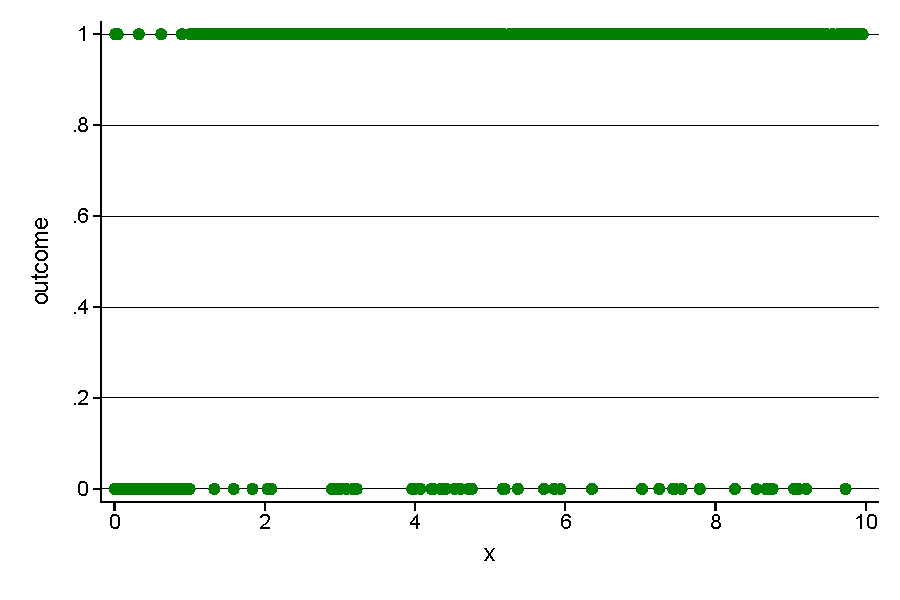
\includegraphics[width=0.7\textwidth]{book_1.pdf}
    \caption{Scatter plot of a binary outcome and a continuous variable x.}
    \label{fig:scatterlinear}
\end{figure}

The graph looks different from the scatter plots that we are used to. This is because the variable outcome, which is the dependent variable, can only take on two values, either a zero or a one. This is why the dots lie 
along one of two lines, the outcome equal zero line and the outcome equal one line. The graph, however, can be informative, as shown in Figure ~\ref{fig:scatterlowess}, which plots the loess curve of the data. A loess plot is simply a smoothed 
scatter plot. Therefore, it allows us to visualize the relationship when the scatter plot is not very clear. This is an extremely useful graph when the variable on the y-axis is binary. As you can see from Figure 4, the 
curve initially increases with increasing values of the dependent variable x, and then levels of when x reaches a value of four. Therefore, we conclude that the relationship between the logit function and the independent 
variable x is not linear.

\begin{stlog}\input{book_2.log.tex}\end{stlog}
\begin{figure}[h]
    \centering
    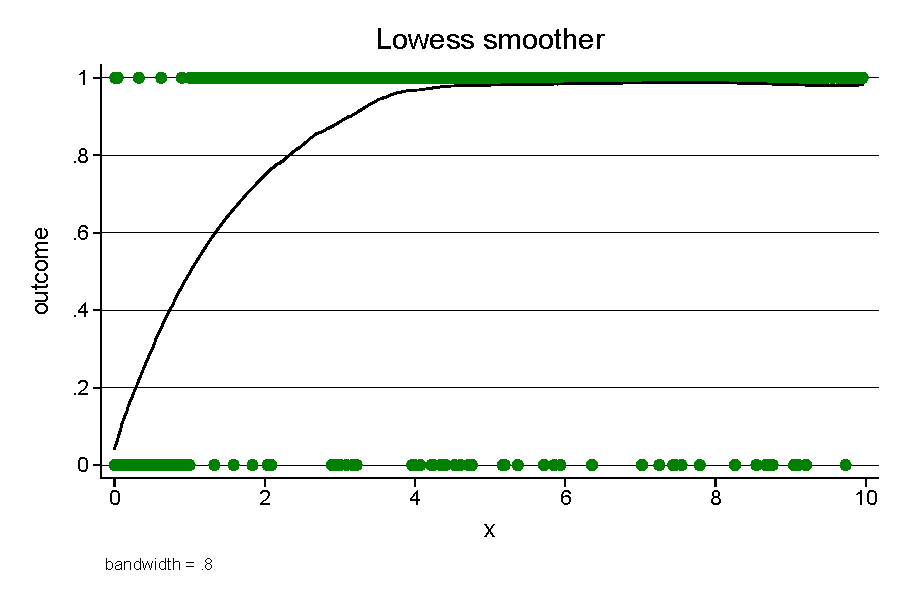
\includegraphics[width=0.7\textwidth]{book_2.pdf}
    \caption{Scatter plot of a binary outcome and a continuous variable x.}
    \label{fig:scatterlowess}
\end{figure}
\paragraph{Linearity of Slopes} 
Another graphical test is the linearity of the slopes test. The idea behind this test is that the independent variable x is categorized. This means that instead of having a continuous independent variable, we end up 
with a categorical variable. Assume for example that we want to categorize the variable age, where age is between 18 years and 60 years. We create a new variable that takes on the value of zero when age is between 18 and 
30, the value one when age is between 30 and 40, the value two when age is between 40 and 50, and the value three when age is greater than 50 (Table ~\ref{table:categorize}). 
\begin{table}[h!t]
	\caption{Categorizing a continuous variable.} \label{table:categorize}
	\centering
	\begin{tabular}{c c}
	\hline
	\bf Categorized age & \bf Age \\
	\hline 
	0 & 18$\leq$age$<$30 \\
	1 & 30$\leq$age$<$40 \\
	2 & 40$\leq$age$<$50 \\
	3 & 50$\leq$age \\
	\hline
	\end{tabular}
\end{table} 
Once we have our new categorized variable, we can fit a logistic regression with the categorized variable as the independent variable. Therefore, instead of having a continuous variable in the model we now have a categorical 
variable. We have already seen how to interpret the results obtained from including a categorical variable. Once the model is fit, we plot a graph of the predicted value of the logit function and the different levels of 
the categorical variable. Figure ~\ref{fig:linearityofslopes} shows the graph that is produced for the same data that was used to produce Figure ~\ref{fig:scatterlowess}, where the independent variable x has been categorized and named xcat. Since when we fit the logistic 
model we obtained the value of the coefficient for each level, we calculate the value of the logit function for each coefficient. If the relationship between the independent variable and the logit function is linear, 
then the graph should resemble a line. This is clearly not the case. In fact, there is a considerable amount of similarity between Figure ~\ref{fig:scatterlowess} and Figure ~\ref{fig:linearityofslopes}. 

\begin{stlog}\input{book_3.log.tex}\end{stlog}
\begin{figure}[h]
    \centering
    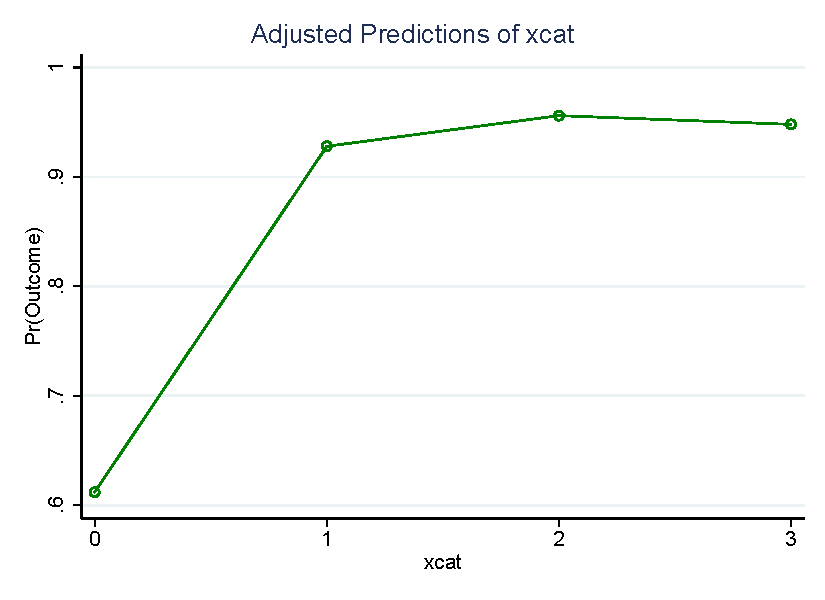
\includegraphics[width=0.7\textwidth]{book_3.pdf}
    \caption{Linearity of slopes test.}
    \label{fig:linearityofslopes}
\end{figure}
\section{Selection of Independent Variables}
An important issue that we face when we have a number of independent variables is how to decide which variables to add to the model and in what order. There are generally four ways to do this. 
The first three all rely on an algorithm and you are advised not to trust them. This is a very important point. You should never let the computer pick the independent variables. However, the three methods 
will be described since many statistical packages allow the user to use them. In addition, I do not think that there is anything wrong with using them as an investigative tool, i.e. in order to get an idea 
of what independent variables are significant and which are not. The first selection method is referred to as forward selection. As the name suggests, this method adds independent variables one step at a time. 
Originally, we start with no independent variables. The algorithm then adds one of the variables. If the p-value of that variable turns out to be less than 0.05, the variable is kept in the model. The algorithm 
then selects another variable and adds it to the model. These models are repeated until there are no further independent variables left.

The second selection method is referred to as backward elimination. As you can imagine, we start with a model that includes all possible independent variables. The algorithm them selects the least significant 
independent variable (the one with the highest p-value). If the p-value of the selected independent variable is greater than 0.05 (which means that it is not significant) the variable is removed. The algorithm 
then repeats and selects the least significant variables from the ones that are still in the model. These steps are repeated until all variables that are included in the model have p-values that are less than 0.05 
(which means that they are all significant).

The third selection method is referred to as stepwise regression. This method is a combination of the previous two. The model starts in forward mode with no independent variables. The algorithm selects the most 
significant independent variable and adds in to the model. Next, the algorithm goes into backward mode by checking to see whether any variable can be eliminated. Next, the algorithm goes back into forward mode 
and selects a variable from the pool of remaining variables, and then it goes back into backward mode. This process continues until there are no more variables to be added or dropped.

As I said, the above three algorithms should not be used to find the final model. You can, however, initially use them in order to get an initial picture of which independent variables are selected and which are not. 
As an initial step, there is nothing wrong with doing this. Ultimately however, you need to rely on the fourth method to select when and how to add the variables, and that method is to use your knowledge. Any good 
research must be informed by theory. The better you understand the theory, the better you can determine which variables to include and which to ignore. In general, we prefer models in which the number of independent 
variables is as small as possible. In linear regression we can rely on the value of R-squared, or adjusted R-squared, when choosing between two models. Although some statistical packages display a statistic that is 
called pseudo R-squared when you run a logistic model, this statistic does not have the same meaning as R-squared does in linear regression, so you should not pay attention to it. We can, however, rely on the AIC and 
BIC statistics when comparing two models. These statistics can be easily calculated by statistical software. When comparing two models, we tend to favor the one with smaller values of both AIC and BIC statistics.

\section{Prediction}
In linear regression, because the left-hand side of the equation is the dependent variable y, we can easily calculate the predicted value of y and then plot it on the y-axis. In logistic regression however, 
the left hand side is not the dependent variable:

$$ \log(\frac{p}{1-p})=ax+b $$

Once we fit the logistic regression model, we are able to calculate the values of a and b. This means that the equation will have one unknown in it, and this unknown is p, which is the probability that the event 
will happen. Since we have one equation and one unknown, we can find the value of the unknown. This means that using logistic regression we can, for each observation, calculate the probability that the event will occur. 
Once we calculate the predicted probability, we can produce graphs in which the predicted probability is plotted on the y-axis and any of the independent variables can be plotted on the x-axis. 
This will allow us to visualize how the probability of an outcome changes with changing values of the independent variable. An example is shown in Figure ~\ref{fig:prediction}, where we can see that the probability of withdrawing from 
a course decreases as the GPA increases.

\begin{stlog}\input{book_4.log.tex}\end{stlog}
\begin{figure}[h]
    \centering
    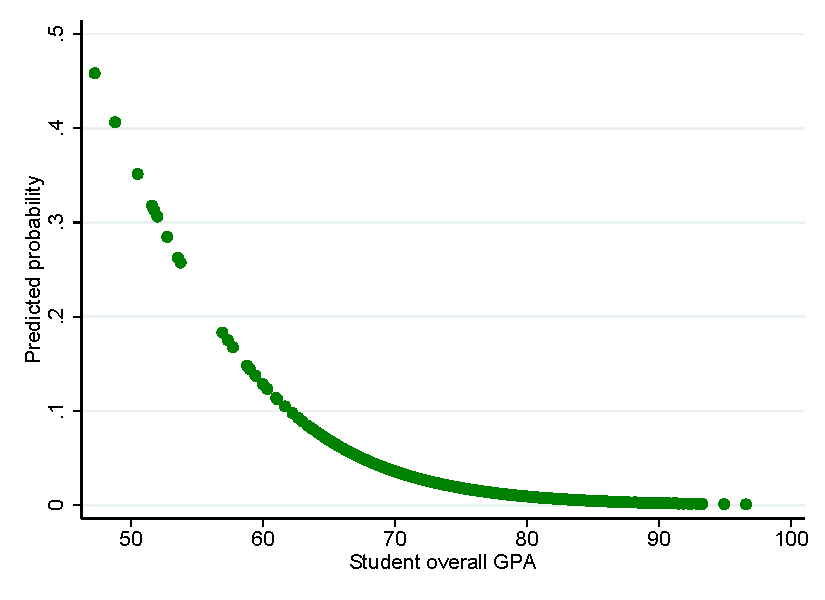
\includegraphics[width=0.7\textwidth]{book_4.pdf}
    \caption{Visualizing the result of logistic regression: Relationship between the probability of withdrawing from a course and student GPAs.}
    \label{fig:prediction}
\end{figure}
\section{Goodness of Fit}
Once we have chosen the variables that we wish to include in the model, we should test how effectively the model describes the outcome variable. There are several ways to do this. In order to illustrate each 
of these ways, consider the data shown in Table ~\ref{table:goodnessoffit}. The output of running a logistic model on this data will be:

$$ \log(\frac{p}{1-p})=2.21(courses)-11.25 $$

By now we know that this means that when the number of courses increases by one, the odds of withdrawing is multiplied by $e^{2.21}=9.12$. The odds, therefore, increase when the course loads increases.
\begin{longtable}[c]{ c c }
	\caption{The dependent variable is outcome and the independent variable is courses.\label{table:goodnessoffit}}\\
		\hline
		\bf Outcome & \bf Courses \\
		\hline
		Withdraw & 6 \\
		Withdraw & 6 \\
		Finish & 4 \\
		Finish & 6 \\
		Finish & 4 \\
		Finish & 3 \\
		Finish & 5 \\
		Finish & 6 \\
		Withdraw & 6 \\
		Finish & 4 \\
		Withdraw & 5 \\
		Finish & 4 \\
		Withdraw & 6 \\
		Withdraw & 5 \\
		Finish & 4 \\
		Finish & 4 \\
		Withdraw & 5 \\
		Withdraw & 6 \\
		Withdraw & 5 \\
		Finish & 4 \\
		Finish & 5 \\
		Withdraw & 6 \\
		Finish & 4 \\
		Finish & 4 \\
		Finish & 5 \\
		Withdraw & 5 \\
		Withdraw & 6 \\
		Withdraw & 5 \\
		Finish & 4 \\
		Finish & 3 \\
		Finish & 4 \\
	\hline
\end{longtable}
\subsection{Likelihood Ratio Test}
This test compares our model with a constant-only model. In other words, this test checks whether the model with the chosen independent variables in significantly better than a model that contains no independent variables. 
If the result of the test is statistically significant (p < 0.05), then we reject the null hypothesis that both models are the same, and we conclude that the model with the independent variables is significantly better. 
Otherwise, if p $\geq$ 0.05, we cannot reject the null hypothesis, thereby we conclude that the model with the added independent variables does not do significantly better than the model with no added variables. With regards to 
the dataset shown in Table ~\ref{table:goodnessoffit}, running a logistic model will result in a p-value that is less than 0.05, thus indicating that the model does significantly better than a constant-only model. 
\subsection{Hosmer-Lemeshow GOF Test}
The Hosmer-Lemeshow test is considered to be one of the best ways to assess the fit of a logistic model. What this test does is that it divides the dataset into groups (usually ten groups), and then compares the 
observed and fitted values within each group. If there is considerable discrepancy between the observed values and the fitted values, the Hosmer-Lemeshow statistic will be large, and this will result in a small p-value. 
What we ideally want to see is that the discrepancy between the observed and the fitted values is small, thereby resulting in a small Hosmer-Lemeshow statistic, which would result in a large p-value. This means that in 
this test, the null hypothesis is that the model fits. If the p-value is less than 0.05, then we reject the null hypothesis and we conclude that the model is not a good fit. 

If we conduct this test on the data in Table ~\ref{table:goodnessoffit}, we will get a p-value of 0.0565 which is only slightly greater than the cut-off value of 0.05. Since the p-value is greater than 0.05, we cannot reject the null 
hypothesis that the model is a good fit.
\subsection{Classification Tables}
An intuitive way of determining whether the model is well-fit or not is to compare the predicted outcome with the actual observed outcome. However, before doing that, we need to determine the point at which the model 
predicts that the outcome will occur. We know that after fitting the logistic model we can calculate the probability that the outcome will occur for each observation. In order for us to be able to construct a classification 
table, we need to determine the probability above which we would consider that the outcome value has occurred. For example, if the predicted probability of the outcome for an observation is 0.88, do we consider that the 
model predicts that the outcome will occur? What about if the probability was 0.52? Usually, a cut-off value of 0.5 is used. If the predicted probability is greater than 0.5, then the model predicts that the dependent 
variable will have a value of one (outcome will occur).

A better way to determine the cutoff value is to actually let the data inform us of the best value to use. The idea here is to calculate the sensitivity and the specificity of the model. Sensitivity represents the 
probability that the model will correctly predict that the outcome has occurred. For example, if the outcome has occurred in 150 of the observations, and the model correctly predicts 140 of them, then the sensitivity 
is 140/150, which is 93.33\%. Specificity on the other hand represents the probability that the model will correctly predict that the outcome has not occurred. For example, if the outcome has not occurred in 200 of the 
observations, and the model correctly predicts 170 of them, then the sensitivity is 170/200, which is 85.00\%. The ideal cutoff value is the one at which sensitivity and specificity are equal.
\begin{table}[h!t]
	\caption{Classification table.} \label{table:classification}
	\centering
	\begin{tabular}{c |c c| c}
	\hline
	{} & \multicolumn{2}{|c|}{Observed} & {} \\
	\hline
	\bf Classified & \bf Outcome = 1 & \bf Outcome = 0 & \bf Total \\
	Outcome = 1 & 7 & 2 & 9 \\
	Outcome = 0 & 6 & 16 & 22 \\
	Total & 13 & 18 & 31 \\
	\hline
	\end{tabular}
\end{table}

As an example, Table ~\ref{table:classification} shows the classification table for the logistic regression model that is fit using the data in Table ~\ref{table:goodnessoffit}. We see that the model correctly predicts seven cases where the observed outcome variable is one, 
which means that the sensitivity is 7/13 which is 53.85\%, and 16 of the cases where the outcome variable is zero, which means that the specificity is 16/18 which is 88.89\%. In two cases, the model predicts a one where the 
observed value is a zero, and in six cases the model predicts a zero where the observed value is one. Therefore, the model correctly classifies (7+16)/31 = 74.19\% of the observations. This is considered to be an acceptable 
value.
\subsection{ROC Analysis}
Another way to test the model fit is to use ROC curves, where we are interested in the area under the curve. This area, which ranges from zero to one, is a measure of the model’s ability to discriminate between 
observations where the outcome of interest is experienced and observations where the outcome of interest is not experienced. The higher the value, the stronger the ability of the model to discriminate. As a general 
guideline:
\begin{itemize}
	\item ROC = 0.5: No ability to discriminate
	\item ROC is between 0.7 and 0.8: Acceptable discrimination
	\item ROC between 0.8 and 0.9: Excellent discrimination
	\item ROC greater than 0.9: Outstanding discrimination
\end{itemize}
If we calculate the area under the ROC curve for the data in Table ~\ref{table:goodnessoffit}, we will find it to be 0.88, thus indicating that the model has an excellent ability to discriminate.
\subsection{Residual Analysis}
Residuals are the difference between the observed outcome and the model’s predicted outcome. As you can imagine, a well-fit model should have small residual values. In linear regression, residual analysis is extremely 
important because linear regression makes strong assumptions about the residuals. In the case of logistic regression, we need to look at the size of the residuals in order to see whether there might be influential 
observations that are biasing our results. 

There are many types of residuals that are used in logistic regression. However, the three most commonly used ones are the standardized residuals, deviance residuals, and the DeltaX residuals. Just like in linear 
regression, these statistics are plotted against the predicted variable in order to visualize the results.
\subsection{Influential Observations}
In linear regression, the three statistics that are used to measure influence are DFBETAS, DFFITS, and Cook’s D statistics. High magnitudes of these statistics indicate that an observation is influential. 
In logistic regression, we use the hat diagonal statistic and the delta-beta influence statistic in order to measure influence. Just as in the case of the residual statistics described above, these statistics are 
plotted against the predicted probabilities in order to visualize the results.

Although there are no fixed-set of rules with regards to determining the values that determine whether an observation is an outlier or whether it is influential, Table ~\ref{table:guidlines} offers some general guidelines that are 
useful in many situations.
\begin{table}[h!t]
	\caption{Guidelines for residual and influence statistics.} \label{table:guidlines}
	\centering
	\begin{tabular}{c c}
	\hline
	\bf Measure & \bf Value above which there might be a problem \\
	\hline
	Deviance residual & Greater than two \\
	DeltaX residual & Greater than four \\
	Hat diagonal statistic & Greater than two times the average hat statistic \\
	Delta-beta influence & Greater than one \\
	\hline
	\end{tabular}
\end{table}

\chapter{Logistic Regression - Application}
We now have the necessary tools that allow us to analyze a dataset where the dependent variable takes on two values. In this section, we will be looking at the dataset logistic\_project.dta. This dataset contains the 
following variables:
\begin{itemize}
	\item withdraw: this is the dependent variable which records whether the student withdrew from the course or finished the course (zero means continued, one means withdraw)
	\item college: whether the student is in the engineering school or the business school (zero means business, one means engineering)
	\item gender: whether the student is a male or a female (zero means female, one means male)
	\item gpa: overall GPA of the student
	\item semester: records whether the course was taken in the spring, fall, or summer semester (zero means fall, one means spring, two means summer)
	\item level: records whether the level of the course (zero means remedial, one means one-hundred level course, two means two-hundred level course, three means three-hundred level course, 
			four means four-hundred level course, and five means five-hundred level course)
\end{itemize}
\section{Univariable Tests}
The first thing that we should do when conducting regression analysis is to perform univariate analysis, where we try and uncover whether there is a relationship between the dependent variable and each independent 
variable separately. Once we have a good idea about the nature of these individual relationships, we can start building the model.
\subsection{Continuous Variables}
In linear regression, when we have a continuous independent variable, we start our analysis by plotting a scatter plot. Graphs are also useful as a starting step in logistic regression, but their shape is 
different from what we are used to due to the nature of the dependent variable. For example, let us tell Stata to produce a scatter plot of the dependent variable withdraw and the continuous independent variable GPA:

\begin{stlog}. scatter withdraw gpa
{\smallskip}
\end{stlog}
\begin{figure}[h]
    \centering
    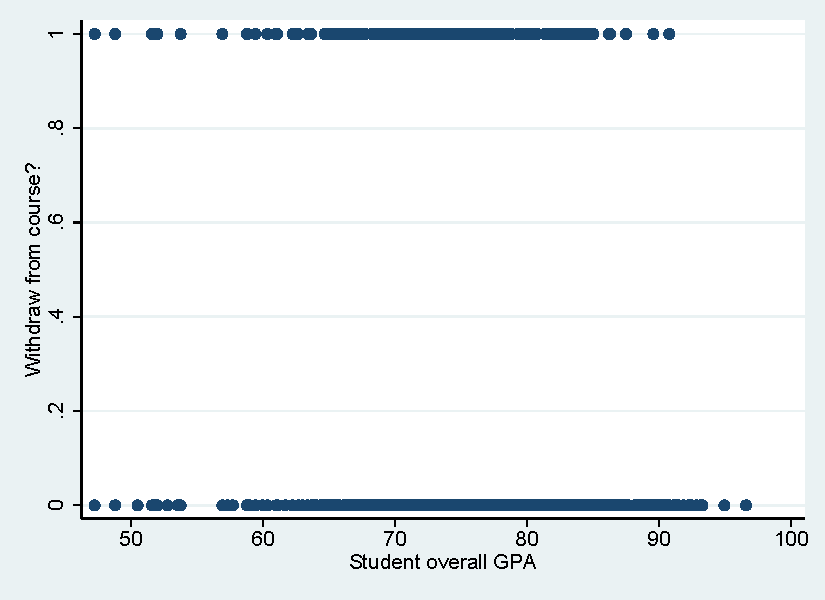
\includegraphics[width=0.7\textwidth]{book_5.pdf}
    \caption{Scatter plot of withdraw and GPA.}
    \label{fig:scatterplot}
\end{figure}

The graph produced by the command is shown in Figure ~\ref{fig:scatterplot}. The reason that the graph looks different is that the variable withdraw can only take on two values, either a zero or a one. This is why the dots lie along 
one of two lines, the withdraw equal zero line and the withdraw equal one line. The graph, however, is informative. Notice, for example, that the students who have a value of one for the withdraw variable 
(these are the students who withdraw from the course) tend to have a GPA that is lower than 85. Students with higher GPAs do not seem to withdraw from courses. However, this does not mean that all students 
with a low GPA withdraw. If you look at the lower horizontal line, we see that the range of GPAs is very wide. We have students who have very low GPAs but who didn’t withdraw from the course, we have students 
with average GPAs who did not withdraw from the course, and we have students with very high GPAs who did not withdraw from the course. The difference between the two horizontal lines is that there is an 
absence of very high GPAs in the line at the top.

We can investigate this further by telling Stata to calculate the average GPA for students who withdraw from courses and then to compare it to the GPA of students who do not withdraw:

\begin{stlog}. by withdraw, sort: summarize gpa
{\smallskip}
\HLI{80}
-> withdraw = No withdraw
{\smallskip}
    Variable {\VBAR}        Obs        Mean    Std. Dev.       Min        Max
\HLI{13}{\PLUS}\HLI{57}
         gpa {\VBAR}     24,656    77.38047    6.622922      47.25      96.59
{\smallskip}
\HLI{80}
-> withdraw = Withdraw
{\smallskip}
    Variable {\VBAR}        Obs        Mean    Std. Dev.       Min        Max
\HLI{13}{\PLUS}\HLI{57}
         gpa {\VBAR}        504    71.18786    6.447055      47.25      90.78
{\smallskip}
{\smallskip}
\end{stlog}

The summarize command tells Stata to display summary statistics about the variable GPA. We use the by command in order to tell Stata to produce the statistics separately for different groups. In our case, 
the groups are determined by the variable withdraw. So we are basically telling Stata to calculate the summary statistics of GPA twice, once for students who have a value of zero for withdraw, and another 
time for students who have a value of one for withdraw. We can see that the average GPA of students who did not withdraw is 77.38 while the average 
for students who did withdraw is 71.19.

We next fit a logistic model where the only independent variable is GPA:

\begin{stlog}. logistic withdraw gpa
{\smallskip}
Logistic regression                             Number of obs     =     25,160
                                                LR chi2(1)        =     425.42
                                                Prob > chi2       =     0.0000
Log likelihood = -2257.0651                     Pseudo R2         =     0.0861
{\smallskip}
\HLI{13}{\TOPT}\HLI{64}
    withdraw {\VBAR} Odds Ratio   Std. Err.      z    P>|z|     [95\% Conf. Interval]
\HLI{13}{\PLUS}\HLI{64}
         gpa {\VBAR}   .8718886   .0057075   -20.94   0.000     .8607737    .8831471
       _cons {\VBAR}     550.52   259.6654    13.38   0.000     218.4159    1387.592
\HLI{13}{\BOTT}\HLI{64}
Note: _cons estimates baseline odds.
{\smallskip}
\end{stlog}

The logistic command is used to tell Stata to fit a logistic regression model. The command is directly followed by the name of the dependent variable and then by the independent variable. 
The output displays the odds ratio. The value of this odds ratio indicates that an increase of one-unit in the GPA causes the odds to be multiplied by 0.87. This means that the odds decrease by 13\%.

We can tell Stata to display the coefficient by specifying the coef option:

\begin{stlog}. logistic withdraw gpa, coef
{\smallskip}
Logistic regression                             Number of obs     =     25,160
                                                LR chi2(1)        =     425.42
                                                Prob > chi2       =     0.0000
Log likelihood = -2257.0651                     Pseudo R2         =     0.0861
{\smallskip}
\HLI{13}{\TOPT}\HLI{64}
    withdraw {\VBAR}      Coef.   Std. Err.      z    P>|z|     [95\% Conf. Interval]
\HLI{13}{\PLUS}\HLI{64}
         gpa {\VBAR}  -.1370936   .0065461   -20.94   0.000    -.1499237   -.1242635
       _cons {\VBAR}   6.310863    .471673    13.38   0.000     5.386401    7.235325
\HLI{13}{\BOTT}\HLI{64}
{\smallskip}
\end{stlog}

The value of the coefficient is -0.1371. We already know that the odds ratio is $e^{-0.1371}=0.87$, which is the odds ratio displayed when we ran the model without the coef option.

The output also shows that the p-value of GPA is less than 0.05, indicating that the result is significant. Therefore, it seems that including the variable in the model is a good idea. However, as 
discussed in the theory section of this course, when we have continuous variables we need to test the assumption of linearity. We know that the form of the logistic model is:

$$ \log(\frac{p}{1-p})=ax+b $$

This means that the independent variable is linear with respect to the logit function. As also discussed in the theory section, there are three ways to test this assumption: the Box-Tidwell test, 
the loess curve, and the linearity of sloped test. We will perform each of these three tests.
\subsubsection{Box-Tidwell Test}
To perform this test we need to create a new variable and to include this variable in the logistic regression model:

\begin{stlog}. gen boxtid = gpa*ln(gpa)
{\smallskip}
. logistic withdraw gpa boxtid
{\smallskip}
Logistic regression                             Number of obs     =     25,160
                                                LR chi2(2)        =     442.63
                                                Prob > chi2       =     0.0000
Log likelihood = -2248.4614                     Pseudo R2         =     0.0896
{\smallskip}
\HLI{13}{\TOPT}\HLI{64}
    withdraw {\VBAR} Odds Ratio   Std. Err.      z    P>|z|     [95\% Conf. Interval]
\HLI{13}{\PLUS}\HLI{64}
         gpa {\VBAR}   4.819065   2.114356     3.58   0.000     2.039387    11.38744
      boxtid {\VBAR}   .7209326   .0605389    -3.90   0.000     .6115284    .8499095
       _cons {\VBAR}   1.20e-07   6.88e-07    -2.78   0.005     1.59e-12    .0090799
\HLI{13}{\BOTT}\HLI{64}
Note: _cons estimates baseline odds.
{\smallskip}
\end{stlog}

The new variable is the product of GPA and the log function of GPA. Since the newly created variable is significant (the p-value is less than 0.05), the result indicates that the relationship between 
the logit function and the variable GPA is not linear.
\subsubsection{Loess Curve}
We next produce the loess curve of the outcome variable, which is withdraw, and the continuous variable, which is GPA:

\begin{stlog}. lowess withdraw gpa, logit
{\smallskip}
\end{stlog}
\begin{figure}[h]
    \centering
    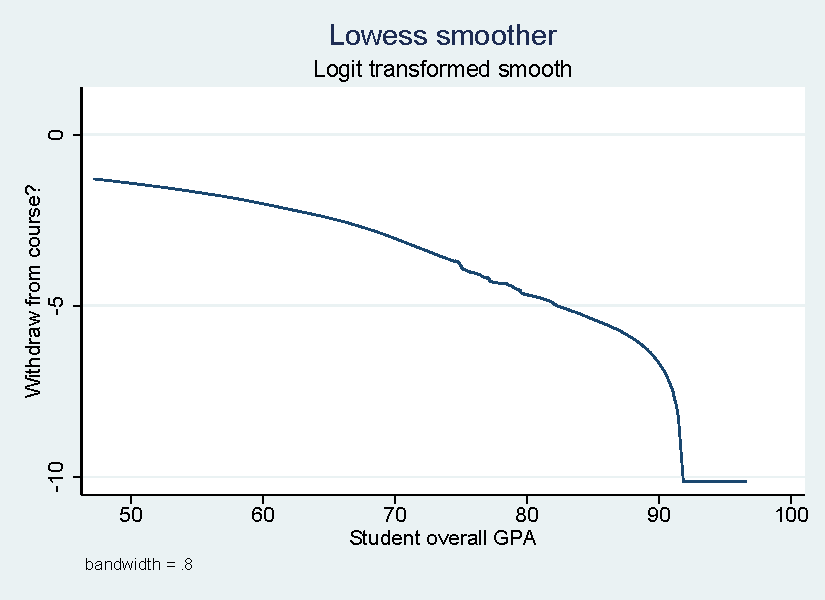
\includegraphics[width=0.7\textwidth]{book_10.pdf}
    \caption{Loess curve of withdraw and GPA.}
    \label{fig:lowesstest}
\end{figure}

Notice that we specified the logit option. This option tells Stata to produce a loess curve in terms of the log of the odds ratio, since we are testing the linearity of GPA with respect to the logit function. 
The result of running the command in shown in Figure ~\ref{fig:lowesstest}. The curve clearly shows that the relationship is not linear, thus providing extra evidence.
\subsubsection{Linearity of Slopes Test}
In order to perform the linearity of slopes test, we need to categorize the continuous variable GPA. Stata provides a very useful command for this purpose:

\begin{stlog}. egen gpacat = cut(gpa), at(40(10)100)
{\smallskip}
\end{stlog}

The egen command is an extension to the generate command. It allows the user to generate new variables using a set of functions. In this case, we are using the cut()function. The command is basically telling 
Stata to generate a new variable, which we named gpacat, by cutting the variable GPA into groups, which are specified in the at() option. This option is telling Stata to group observations with a GPA between 40 
and 50 in one group, 50 and 60 in a second group, 60 and 70 in a third group, 70 and 80 in a fourth group, 80 and 90 in a fifth group, and finally 90 and 100 in a sixth group.

We can take a closer look at our newly created variable:

\begin{stlog}. tabulate gpacat
{\smallskip}
     gpacat {\VBAR}      Freq.     Percent        Cum.
\HLI{12}{\PLUS}\HLI{35}
         40 {\VBAR}         19        0.08        0.08
         50 {\VBAR}        154        0.61        0.69
         60 {\VBAR}      2,009        7.98        8.67
         70 {\VBAR}     14,912       59.27       67.94
         80 {\VBAR}      7,212       28.66       96.61
         90 {\VBAR}        854        3.39      100.00
\HLI{12}{\PLUS}\HLI{35}
      Total {\VBAR}     25,160      100.00
{\smallskip}
\end{stlog}

We see that there are four groups where each contains roughly the same number of observations. The groups are in order. This means that group zero contains the GPAs which are in the bottom quartile and group 
three contains the GPAs which are in the top quartile.

Now that we have our categorical variable, we include it by itself in a logistic model:

\begin{stlog}. logistic withdraw i.gpacat
{\smallskip}
Logistic regression                             Number of obs     =     25,160
                                                LR chi2(5)        =     321.65
                                                Prob > chi2       =     0.0000
Log likelihood = -2308.9538                     Pseudo R2         =     0.0651
{\smallskip}
\HLI{13}{\TOPT}\HLI{64}
    withdraw {\VBAR} Odds Ratio   Std. Err.      z    P>|z|     [95\% Conf. Interval]
\HLI{13}{\PLUS}\HLI{64}
      gpacat {\VBAR}
         50  {\VBAR}   .5597015   .3423477    -0.95   0.343     .1687756    1.856109
         60  {\VBAR}   .2509294   .1430813    -2.42   0.015     .0820714    .7672047
         70  {\VBAR}   .0814491   .0460666    -4.43   0.000     .0268817    .2467833
         80  {\VBAR}   .0188127   .0110433    -6.77   0.000     .0059537    .0594453
         90  {\VBAR}   .0043962   .0050468    -4.73   0.000     .0004634    .0417097
             {\VBAR}
       _cons {\VBAR}   .2666667   .1500617    -2.35   0.019     .0885056    .8034643
\HLI{13}{\BOTT}\HLI{64}
Note: _cons estimates baseline odds.
{\smallskip}
\end{stlog}

Notice that we use the i prefix. This is how we tell Stata that this is a categorical variable. Otherwise, Stata will treat the variable like a continuous variable that takes on values from zero to three. 

We would next want to produce a graph in order to see whether the relationship is linear or not. To do this we take advantage of Stata’s excellent margins and marginsplot commands. 
These commands make producing graphs very easy. The margins command calculates the values while the marginsplot command plots them. Since we are running a logistic model, the margins 
command calculates the predicted probabilities. This, however, is not what we want, since we want to check for linearity by plotting the logit function against the categorical variable. 
Therefore, we need to tell Stata to calculate the value of the logit function at each value of the categorical variable by including the predict(xb) option:

\begin{stlog}. margins gpacat, predict(xb)
{\smallskip}
Adjusted predictions                            Number of obs     =     25,160
Model VCE    : OIM
{\smallskip}
Expression   : Linear prediction (log odds), predict(xb)
{\smallskip}
\HLI{13}{\TOPT}\HLI{64}
             {\VBAR}            Delta-method
             {\VBAR}     Margin   Std. Err.      z    P>|z|     [95\% Conf. Interval]
\HLI{13}{\PLUS}\HLI{64}
      gpacat {\VBAR}
         40  {\VBAR}  -1.321756   .5627314    -2.35   0.019    -2.424689   -.2188225
         50  {\VBAR}  -1.902108   .2397138    -7.93   0.000    -2.371938   -1.432277
         60  {\VBAR}   -2.70434   .0920194   -29.39   0.000    -2.884694   -2.523985
         70  {\VBAR}  -3.829533   .0567723   -67.45   0.000    -3.940804   -3.718261
         80  {\VBAR}  -5.294978   .1670842   -31.69   0.000    -5.622457   -4.967499
         90  {\VBAR}  -6.748759   1.000586    -6.74   0.000    -8.709871   -4.787647
\HLI{13}{\BOTT}\HLI{64}
{\smallskip}
\end{stlog}

What this command is doing is that it is predicting the value of the logit function at each level of the categorical variable gpacat. We can see that the values for each level of the categorical variable is 
calculated and displayed in the column titled “Margin”. We next use the marginsplot command to plot the values:

\begin{stlog}. marginsplot, noci
{\smallskip}
  Variables that uniquely identify margins: gpacat
{\smallskip}
\end{stlog}
\begin{figure}[h]
    \centering
    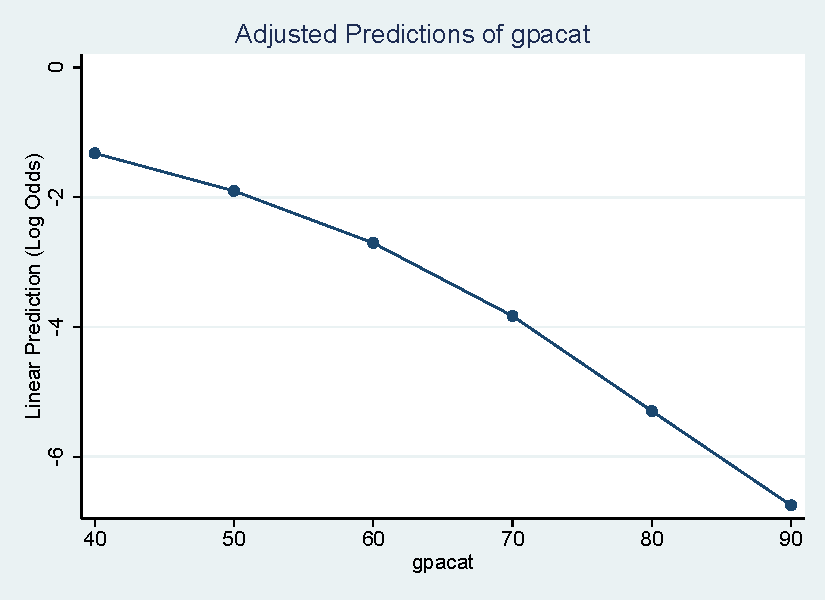
\includegraphics[width=0.7\textwidth]{book_15.pdf}
    \caption{The output of the marginsplot command allows us to test the linearity of the slopes assumption.}
    \label{fig:marginslinearity}
\end{figure}

This command is simply telling Stata to plot the values that it has already calculated when we ran the margins command. The graph is shown in Figure ~\ref{fig:marginslinearity}. 
Once again, the nonlinearity is evident in the graph as it curves downward.
\subsection{Including a Quadratic Term}
Now that we have seen that there is nonlinearity when it comes to the independent variable GPA, we need to do something to account for this nonlinearity. One way to include nonlinearity in a 
regression model is to add a quadratic term, where this term is the square of the variable. By including the original variable and the squared term, we will be modeling the following equation:

$$ \log(\frac{p}{1-p})=a_1x^2+a_2x+b $$

There are two ways in which we can do this in Stata. Both produce the same equation, but one makes visualizing the result easy while the other complicates things. We first start with the method that you should not use.
\subsubsection{Generating a New Variable}
In the first method, we created a new variable that we named English2, and we included this variable in the model:

\begin{figure}[h]
    \centering
    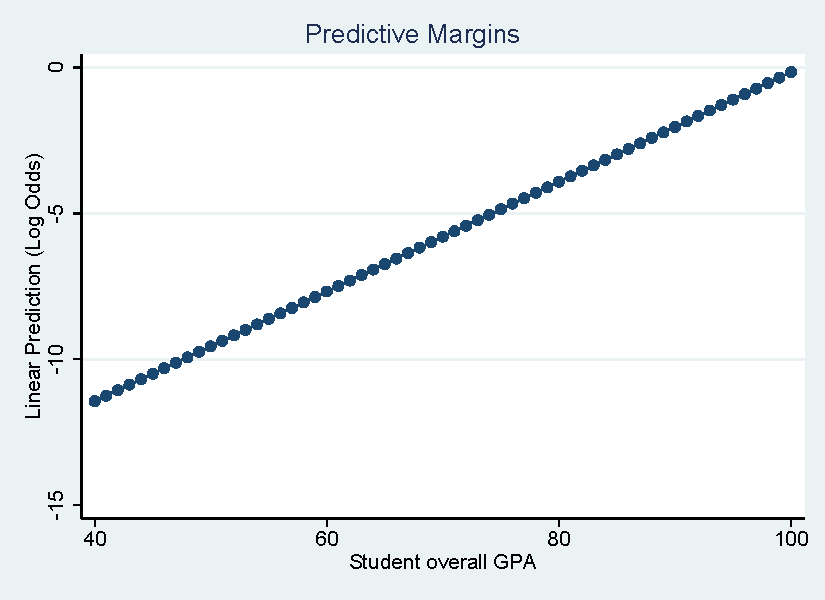
\includegraphics[width=0.7\textwidth]{book_16.pdf}
    \caption{The output of the marginsplot command allows us to test the linearity of the slopes assumption.}
    \label{fig:quadratic1}
\end{figure}
\begin{stlog}. gen gpa2 = gpa*gpa
{\smallskip}
. logistic withdraw gpa gpa2
{\smallskip}
Logistic regression                             Number of obs     =     25,160
                                                LR chi2(2)        =     441.91
                                                Prob > chi2       =     0.0000
Log likelihood = -2248.8207                     Pseudo R2         =     0.0895
{\smallskip}
\HLI{13}{\TOPT}\HLI{64}
    withdraw {\VBAR} Odds Ratio   Std. Err.      z    P>|z|     [95\% Conf. Interval]
\HLI{13}{\PLUS}\HLI{64}
         gpa {\VBAR}   1.206675   .1030634     2.20   0.028     1.020677    1.426568
        gpa2 {\VBAR}   .9976426   .0006178    -3.81   0.000     .9964324    .9988542
       _cons {\VBAR}   .0086151   .0253454    -1.62   0.106      .000027    2.750891
\HLI{13}{\BOTT}\HLI{64}
Note: _cons estimates baseline odds.
{\smallskip}
. margins, at(gpa=(40(1)100)) predict(xb) noatlegend
{\smallskip}
Predictive margins                              Number of obs     =     25,160
Model VCE    : OIM
{\smallskip}
Expression   : Linear prediction (log odds), predict(xb)
{\smallskip}
\HLI{13}{\TOPT}\HLI{64}
             {\VBAR}            Delta-method
             {\VBAR}     Margin   Std. Err.      z    P>|z|     [95\% Conf. Interval]
\HLI{13}{\PLUS}\HLI{64}
         _at {\VBAR}
          1  {\VBAR}  -11.43162   3.223198    -3.55   0.000    -17.74897   -5.114267
          2  {\VBAR}  -11.24375   3.137805    -3.58   0.000    -17.39374   -5.093766
          3  {\VBAR}  -11.05588   3.052413    -3.62   0.000     -17.0385   -5.073264
          4  {\VBAR}  -10.86801   2.967021    -3.66   0.000    -16.68327   -5.052759
          5  {\VBAR}  -10.68015   2.881631    -3.71   0.000    -16.32804   -5.032251
          6  {\VBAR}  -10.49228   2.796243    -3.75   0.000    -15.97281   -5.011742
          7  {\VBAR}  -10.30441   2.710855    -3.80   0.000    -15.61759   -4.991229
          8  {\VBAR}  -10.11654   2.625469    -3.85   0.000    -15.26236   -4.970714
          9  {\VBAR}   -9.92867   2.540085    -3.91   0.000    -14.90715   -4.950195
         10  {\VBAR}  -9.740801   2.454703    -3.97   0.000    -14.55193   -4.929672
         11  {\VBAR}  -9.552933   2.369323    -4.03   0.000    -14.19672   -4.909146
         12  {\VBAR}  -9.365064   2.283945    -4.10   0.000    -13.84151   -4.888614
         13  {\VBAR}  -9.177195   2.198569    -4.17   0.000    -13.48631   -4.868078
         14  {\VBAR}  -8.989326   2.113197    -4.25   0.000    -13.13112   -4.847536
         15  {\VBAR}  -8.801458   2.027828    -4.34   0.000    -12.77593   -4.826988
         16  {\VBAR}  -8.613589   1.942462    -4.43   0.000    -12.42074   -4.806433
         17  {\VBAR}   -8.42572   1.857101    -4.54   0.000    -12.06557   -4.785869
         18  {\VBAR}  -8.237851   1.771744    -4.65   0.000    -11.71041   -4.765296
         19  {\VBAR}  -8.049983   1.686393    -4.77   0.000    -11.35525   -4.744712
         20  {\VBAR}  -7.862114   1.601049    -4.91   0.000    -11.00011   -4.724116
         21  {\VBAR}  -7.674245   1.515712    -5.06   0.000    -10.64499   -4.703505
         22  {\VBAR}  -7.486376   1.430383    -5.23   0.000    -10.28988   -4.682876
         23  {\VBAR}  -7.298508   1.345066    -5.43   0.000    -9.934788   -4.662228
         24  {\VBAR}  -7.110639    1.25976    -5.64   0.000    -9.579724   -4.641554
         25  {\VBAR}   -6.92277   1.174471    -5.89   0.000    -9.224691    -4.62085
         26  {\VBAR}  -6.734901     1.0892    -6.18   0.000    -8.869694   -4.600109
         27  {\VBAR}  -6.547033   1.003953    -6.52   0.000    -8.514745   -4.579321
         28  {\VBAR}  -6.359164   .9187368    -6.92   0.000    -8.159855   -4.558473
         29  {\VBAR}  -6.171295   .8335603    -7.40   0.000    -7.805043   -4.537547
         30  {\VBAR}  -5.983426   .7484373    -7.99   0.000    -7.450337   -4.516516
         31  {\VBAR}  -5.795558   .6633883    -8.74   0.000    -7.095775    -4.49534
         32  {\VBAR}  -5.607689   .5784461    -9.69   0.000    -6.741422   -4.473955
         33  {\VBAR}   -5.41982   .4936656   -10.98   0.000    -6.387387   -4.452253
         34  {\VBAR}  -5.231951   .4091476   -12.79   0.000    -6.033866   -4.430037
         35  {\VBAR}  -5.044083   .3250966   -15.52   0.000     -5.68126   -4.406905
         36  {\VBAR}  -4.856214       .242   -20.07   0.000    -5.330525   -4.381903
         37  {\VBAR}  -4.668345    .161339   -28.94   0.000    -4.984564   -4.352127
         38  {\VBAR}  -4.480476   .0899259   -49.82   0.000    -4.656728   -4.304225
         39  {\VBAR}  -4.292608   .0687979   -62.39   0.000    -4.427449   -4.157766
         40  {\VBAR}  -4.104739   .1263714   -32.48   0.000    -4.352422   -3.857055
         41  {\VBAR}   -3.91687   .2044418   -19.16   0.000    -4.317569   -3.516172
         42  {\VBAR}  -3.729001   .2867285   -13.01   0.000    -4.290979   -3.167024
         43  {\VBAR}  -3.541133   .3704323    -9.56   0.000    -4.267167   -2.815099
         44  {\VBAR}  -3.353264   .4547715    -7.37   0.000      -4.2446   -2.461928
         45  {\VBAR}  -3.165395   .5394481    -5.87   0.000    -4.222694   -2.108096
         46  {\VBAR}  -2.977526   .6243248    -4.77   0.000    -4.201181   -1.753872
         47  {\VBAR}  -2.789658   .7093297    -3.93   0.000    -4.179918   -1.399397
         48  {\VBAR}  -2.601789   .7944219    -3.28   0.001    -4.158827   -1.044751
         49  {\VBAR}   -2.41392   .8795758    -2.74   0.006    -4.137857   -.6899834
         50  {\VBAR}  -2.226051   .9647752    -2.31   0.021    -4.116976   -.3351268
         51  {\VBAR}  -2.038183   1.050009    -1.94   0.052    -4.096163    .0197971
         52  {\VBAR}  -1.850314   1.135269    -1.63   0.103    -4.075401    .3747732
         53  {\VBAR}  -1.662445   1.220551    -1.36   0.173    -4.054681    .7297906
         54  {\VBAR}  -1.474577   1.305849    -1.13   0.259    -4.033994    1.084841
         55  {\VBAR}  -1.286708   1.391162    -0.92   0.355    -4.013334    1.439919
         56  {\VBAR}  -1.098839   1.476485    -0.74   0.457    -3.992697    1.795019
         57  {\VBAR}  -.9109703   1.561819    -0.58   0.560    -3.972078    2.150138
         58  {\VBAR}  -.7231015    1.64716    -0.44   0.661    -3.951476    2.505272
         59  {\VBAR}  -.5352328   1.732508    -0.31   0.757    -3.930886    2.860421
         60  {\VBAR}   -.347364   1.817862    -0.19   0.848    -3.910308     3.21558
         61  {\VBAR}  -.1594953   1.903221    -0.08   0.933    -3.889741     3.57075
\HLI{13}{\BOTT}\HLI{64}
{\smallskip}
. marginsplot, noci
{\smallskip}
  Variables that uniquely identify margins: gpa
{\smallskip}
\end{stlog}

The first command generates a new variable which is the square of GPA. The second command includes both GPA and the newly created variable in the logistic model. The third command tells Stata to calculate 
the values of the logit function since we included the predict(xb) option (The output of the command is very long, so I used the noatlegend option in order to suppress some parts of it). The values are calculated while 
varying the value of GPA from 40 to 100 in increments of one. The fourth command plots the calculated values. The result is shown in Figure ~\ref{fig:quadratic1}.

The output is strange. Our linear model includes a squared term, yet the graph is a straight line. Why? The reason is simply because Stata does not know that the variable gpa2 is the square of the variable GPA. 
Stata includes the variable just like any other independent variable. When an independent variable that is included in the model is not included in the at() option of the margins command, Stata sets the value of 
the variable to the mean. Since the mean of the variable gpa2 is 6013.122, Stata is calculating the following:

GPA=40: $ \log(\frac{p}{1-p})=0.1878687(40)-0.0023602(6013.122)-4.754241 $

GPA=41: $ \log(\frac{p}{1-p})=0.1878687(41)-0.0023602(6013.122)-4.754241 $

GPA=42: $ \log(\frac{p}{1-p})=0.1878687(42)-0.0023602(6013.122)-4.754241 $

.

.

.

GPA=100: $ \log(\frac{p}{1-p})=0.1878687(100)-0.0023602(6013.122)-4.754241 $

Notice that the value of gpa2 is not changing. The variable is fixed at the mean. Stata does not know that when GPA is 40 gpa2 is 40*40, even though this is the formula that we used to generate the variable gpa2.
\subsubsection{Using Interaction Terms}
Let us now include the quadratic term using an interaction term:

\begin{stlog}. logistic withdraw gpa c.gpa\#c.gpa
{\smallskip}
Logistic regression                             Number of obs     =     25,160
                                                LR chi2(2)        =     441.91
                                                Prob > chi2       =     0.0000
Log likelihood = -2248.8207                     Pseudo R2         =     0.0895
{\smallskip}
\HLI{13}{\TOPT}\HLI{64}
    withdraw {\VBAR} Odds Ratio   Std. Err.      z    P>|z|     [95\% Conf. Interval]
\HLI{13}{\PLUS}\HLI{64}
         gpa {\VBAR}   1.206675   .1030634     2.20   0.028     1.020677    1.426568
             {\VBAR}
 c.gpa\#c.gpa {\VBAR}   .9976426   .0006178    -3.81   0.000     .9964324    .9988542
             {\VBAR}
       _cons {\VBAR}   .0086151   .0253454    -1.62   0.106      .000027    2.750898
\HLI{13}{\BOTT}\HLI{64}
Note: _cons estimates baseline odds.
{\smallskip}
\end{stlog}

Notice that this command does not use any new variable. Instead, it includes the term c.gpa\#c.gpa. This term is how we tell Stata to include a variable that is GPA x GPA. The prefix c tells Stata that the variable GPA is 
continuous. The output from running this command is exactly the same as the output from running the command where the quadratic term was included by generating the variable gpa2. The only difference is in the name of 
the variable in the output. Notice that the interaction term is statistically significant (p-value < 0.05).

Now that we have fit the logistic model, let us generate the graph:

\begin{figure}[h]
    \centering
    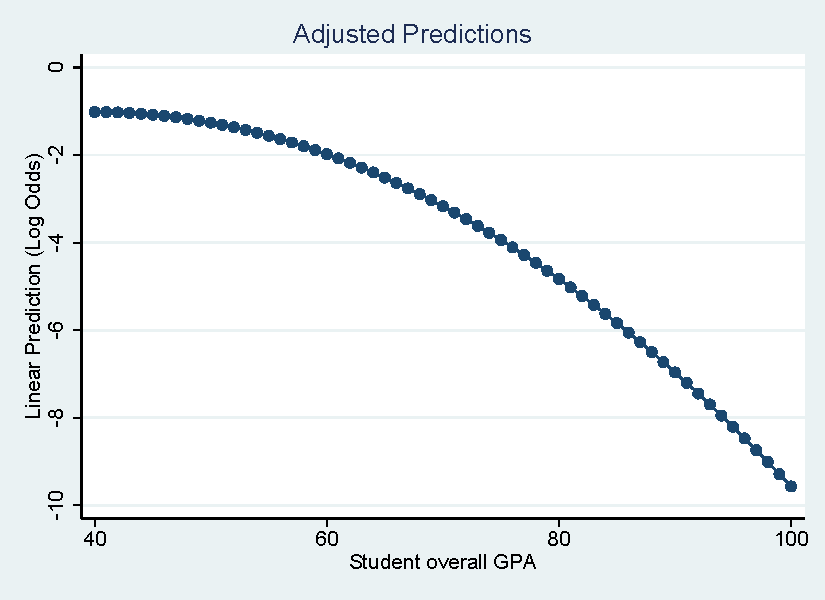
\includegraphics[width=0.7\textwidth]{book_18.pdf}
    \caption{The graph produced when the quadratic term is included as an interaction term.}
    \label{fig:quadratic2}
\end{figure}
\begin{stlog}. margins, at(gpa=(40(1)100)) predict(xb) noatlegend
{\smallskip}
Adjusted predictions                            Number of obs     =     25,160
Model VCE    : OIM
{\smallskip}
Expression   : Linear prediction (log odds), predict(xb)
{\smallskip}
\HLI{13}{\TOPT}\HLI{64}
             {\VBAR}            Delta-method
             {\VBAR}     Margin   Std. Err.      z    P>|z|     [95\% Conf. Interval]
\HLI{13}{\PLUS}\HLI{64}
         _at {\VBAR}
          1  {\VBAR}    -1.0158   .5358692    -1.90   0.058    -2.066084    .0344847
          2  {\VBAR}  -1.019107   .5013986    -2.03   0.042     -2.00183   -.0363834
          3  {\VBAR}  -1.027134   .4682042    -2.19   0.028    -1.944797   -.1094706
          4  {\VBAR}  -1.039882   .4362902    -2.38   0.017    -1.894995   -.1847686
          5  {\VBAR}   -1.05735   .4056616    -2.61   0.009    -1.852432   -.2622676
          6  {\VBAR}  -1.079538   .3763241    -2.87   0.004     -1.81712   -.3419566
          7  {\VBAR}  -1.106447   .3482839    -3.18   0.001    -1.789071   -.4238232
          8  {\VBAR}  -1.138076   .3215484    -3.54   0.000      -1.7683   -.5078532
          9  {\VBAR}  -1.174426   .2961258    -3.97   0.000    -1.754822   -.5940302
         10  {\VBAR}  -1.215496   .2720254    -4.47   0.000    -1.748656    -.682336
         11  {\VBAR}  -1.261286   .2492578    -5.06   0.000    -1.749823     -.77275
         12  {\VBAR}  -1.311797   .2278346    -5.76   0.000    -1.758345   -.8652497
         13  {\VBAR}  -1.367028   .2077682    -6.58   0.000    -1.774247   -.9598102
         14  {\VBAR}   -1.42698    .189072    -7.55   0.000    -1.797554   -1.056406
         15  {\VBAR}  -1.491652   .1717591    -8.68   0.000    -1.828294    -1.15501
         16  {\VBAR}  -1.561044   .1558415   -10.02   0.000    -1.866488     -1.2556
         17  {\VBAR}  -1.635157   .1413281   -11.57   0.000    -1.912155   -1.358159
         18  {\VBAR}   -1.71399   .1282217   -13.37   0.000      -1.9653    -1.46268
         19  {\VBAR}  -1.797544   .1165149   -15.43   0.000    -2.025909   -1.569179
         20  {\VBAR}  -1.885817   .1061851   -17.76   0.000    -2.093936   -1.677699
         21  {\VBAR}  -1.978812   .0971879   -20.36   0.000    -2.169296   -1.788327
         22  {\VBAR}  -2.076526   .0894519   -23.21   0.000    -2.251849   -1.901204
         23  {\VBAR}  -2.178961   .0828746   -26.29   0.000    -2.341393    -2.01653
         24  {\VBAR}  -2.286117   .0773229   -29.57   0.000    -2.437667   -2.134567
         25  {\VBAR}  -2.397993    .072639   -33.01   0.000    -2.540362   -2.255623
         26  {\VBAR}  -2.514589   .0686516   -36.63   0.000    -2.649144   -2.380034
         27  {\VBAR}  -2.635905   .0651919   -40.43   0.000    -2.763679   -2.508132
         28  {\VBAR}  -2.761942   .0621106   -44.47   0.000    -2.883677   -2.640208
         29  {\VBAR}    -2.8927   .0592956   -48.78   0.000    -3.008917   -2.776482
         30  {\VBAR}  -3.028177   .0566886   -53.42   0.000    -3.139285    -2.91707
         31  {\VBAR}  -3.168376   .0543021   -58.35   0.000    -3.274806   -3.061945
         32  {\VBAR}  -3.313294   .0522364   -63.43   0.000    -3.415675   -3.210913
         33  {\VBAR}  -3.462933   .0506938   -68.31   0.000    -3.562291   -3.363575
         34  {\VBAR}  -3.617292    .049981   -72.37   0.000    -3.715253   -3.519331
         35  {\VBAR}  -3.776372   .0504804   -74.81   0.000    -3.875312   -3.677432
         36  {\VBAR}  -3.940172   .0525785   -74.94   0.000    -4.043224    -3.83712
         37  {\VBAR}  -4.108692   .0565694   -72.63   0.000    -4.219566   -3.997818
         38  {\VBAR}  -4.281933   .0625908   -68.41   0.000    -4.404609   -4.159257
         39  {\VBAR}  -4.459894   .0706312   -63.14   0.000    -4.598329    -4.32146
         40  {\VBAR}  -4.642576   .0805884   -57.61   0.000    -4.800526   -4.484626
         41  {\VBAR}  -4.829978   .0923305   -52.31   0.000    -5.010942   -4.649013
         42  {\VBAR}    -5.0221   .1057328   -47.50   0.000    -5.229333   -4.814868
         43  {\VBAR}  -5.218943    .120692   -43.24   0.000    -5.455495   -4.982391
         44  {\VBAR}  -5.420506   .1371278   -39.53   0.000    -5.689272   -5.151741
         45  {\VBAR}   -5.62679   .1549801   -36.31   0.000    -5.930545   -5.323034
         46  {\VBAR}  -5.837793   .1742043   -33.51   0.000    -6.179228   -5.496359
         47  {\VBAR}  -6.053518   .1947672   -31.08   0.000    -6.435254   -5.671781
         48  {\VBAR}  -6.273962   .2166444   -28.96   0.000    -6.698578   -5.849347
         49  {\VBAR}  -6.499128   .2398178   -27.10   0.000    -6.969162   -6.029093
         50  {\VBAR}  -6.729013   .2642735   -25.46   0.000    -7.246979   -6.211046
         51  {\VBAR}  -6.963619   .2900013   -24.01   0.000    -7.532011   -6.395227
         52  {\VBAR}  -7.202945   .3169933   -22.72   0.000     -7.82424    -6.58165
         53  {\VBAR}  -7.446992   .3452435   -21.57   0.000    -8.123656   -6.770327
         54  {\VBAR}  -7.695759   .3747473   -20.54   0.000     -8.43025   -6.961267
         55  {\VBAR}  -7.949246   .4055011   -19.60   0.000    -8.744013   -7.154478
         56  {\VBAR}  -8.207454    .437502   -18.76   0.000    -9.064942   -7.349966
         57  {\VBAR}  -8.470382   .4707479   -17.99   0.000    -9.393031   -7.547733
         58  {\VBAR}   -8.73803   .5052372   -17.29   0.000    -9.728277   -7.747784
         59  {\VBAR}  -9.010399   .5409683   -16.66   0.000    -10.07068   -7.950121
         60  {\VBAR}  -9.287489   .5779403   -16.07   0.000    -10.42023   -8.154746
         61  {\VBAR}  -9.569298   .6161523   -15.53   0.000    -10.77693   -8.361662
\HLI{13}{\BOTT}\HLI{64}
{\smallskip}
. marginsplot, noci
{\smallskip}
  Variables that uniquely identify margins: gpa
{\smallskip}
\end{stlog}

The output is shown in Figure ~\ref{fig:quadratic2}. The difference is clear. This correct graph shows how the logit function decreases with increasing values of GPA. By using the c.gpa\#c.gpa notation, 
we have explicitly told Stata that the second term is the squared of GPA. Stata is now calculating the following:

GPA=40: $ \log(\frac{p}{1-p})=0.1878687(40)-0.0023602(40^2)-4.754241 $

GPA=41: $ \log(\frac{p}{1-p})=0.1878687(41)-0.0023602(41^2)-4.754241 $

GPA=42: $ \log(\frac{p}{1-p})=0.1878687(42)-0.0023602(42^2)-4.754241 $

.

.

.

GPA=100: $ \log(\frac{p}{1-p})=0.1878687(100)-0.0023602(100^2)-4.754241 $

This example illustrates why you should always use interaction terms.
\subsection{Binary Variables} 
Now that we have seen how to analyze the relationship between the binary dependent variable and a continuous independent variable, we move onto other types of variables. Looking at our dataset, we notice 
that the variables gender and college are binary. Both take on two values. While graphs are used to investigate the relationship when a continuous variable is involved, contingency tables are used to investigate 
the relationship when the independent variable is binary.

We start by looking at the variable gender. The following command creates a cross tabulation of the variables withdraw and gender:

\begin{stlog}. tabulate gender withdraw
{\smallskip}
           {\VBAR} Withdraw from course?
    Gender {\VBAR} No withdr   Withdraw {\VBAR}     Total
\HLI{11}{\PLUS}\HLI{22}{\PLUS}\HLI{10}
    female {\VBAR}     7,957         76 {\VBAR}     8,033 
      male {\VBAR}    16,699        428 {\VBAR}    17,127 
\HLI{11}{\PLUS}\HLI{22}{\PLUS}\HLI{10}
     Total {\VBAR}    24,656        504 {\VBAR}    25,160 
{\smallskip}
\end{stlog}

We notice that the table includes frequencies. It would also be useful if we were able to see the percent of females who withdrew from a course and the percent of males who withdrew. This can be done by 
specifying the row option which tells Stata to calculate the percentages in each row:

\begin{stlog}. tabulate gender withdraw, row
{\smallskip}
{\TLC}\HLI{16}{\TRC}
{\VBAR} Key            {\VBAR}
{\LFTT}\HLI{16}{\RGTT}
{\VBAR}   {\sltt{frequency}}    {\VBAR}
{\VBAR} {\sltt{row percentage}} {\VBAR}
{\BLC}\HLI{16}{\BRC}
{\smallskip}
           {\VBAR} Withdraw from course?
    Gender {\VBAR} No withdr   Withdraw {\VBAR}     Total
\HLI{11}{\PLUS}\HLI{22}{\PLUS}\HLI{10}
    female {\VBAR}     7,957         76 {\VBAR}     8,033 
           {\VBAR}     99.05       0.95 {\VBAR}    100.00 
\HLI{11}{\PLUS}\HLI{22}{\PLUS}\HLI{10}
      male {\VBAR}    16,699        428 {\VBAR}    17,127 
           {\VBAR}     97.50       2.50 {\VBAR}    100.00 
\HLI{11}{\PLUS}\HLI{22}{\PLUS}\HLI{10}
     Total {\VBAR}    24,656        504 {\VBAR}    25,160 
           {\VBAR}     98.00       2.00 {\VBAR}    100.00 
{\smallskip}
\end{stlog}

We see that 0.95\% of females withdrew from courses as opposed to the 2.50\% of males. This result indicates that there seems to be a difference between the two groups. To verify this, we fit a logistic model:

\begin{stlog}. logistic withdraw i.gender
{\smallskip}
Logistic regression                             Number of obs     =     25,160
                                                LR chi2(1)        =      76.62
                                                Prob > chi2       =     0.0000
Log likelihood = -2431.4659                     Pseudo R2         =     0.0155
{\smallskip}
\HLI{13}{\TOPT}\HLI{64}
    withdraw {\VBAR} Odds Ratio   Std. Err.      z    P>|z|     [95\% Conf. Interval]
\HLI{13}{\PLUS}\HLI{64}
      gender {\VBAR}
       male  {\VBAR}   2.683423   .3360166     7.88   0.000     2.099433    3.429857
       _cons {\VBAR}   .0095513   .0011008   -40.35   0.000     .0076201    .0119721
\HLI{13}{\BOTT}\HLI{64}
Note: _cons estimates baseline odds.
{\smallskip}
\end{stlog}

Notice that we include the i prefix in the binary variable. The output shows that the odds ratios is 2.68. This means that the odds of males are 2.68 times the odds of females. The result is significant since 
the p-value is less than 0.05. Therefore, when building our final model, it would make sense to include this variable.

We next perform the same analysis for the variable college:

\begin{stlog}. tab college withdraw, row
{\smallskip}
{\TLC}\HLI{16}{\TRC}
{\VBAR} Key            {\VBAR}
{\LFTT}\HLI{16}{\RGTT}
{\VBAR}   {\sltt{frequency}}    {\VBAR}
{\VBAR} {\sltt{row percentage}} {\VBAR}
{\BLC}\HLI{16}{\BRC}
{\smallskip}
            {\VBAR} Withdraw from course?
    College {\VBAR} No withdr   Withdraw {\VBAR}     Total
\HLI{12}{\PLUS}\HLI{22}{\PLUS}\HLI{10}
   Business {\VBAR}     9,079        219 {\VBAR}     9,298 
            {\VBAR}     97.64       2.36 {\VBAR}    100.00 
\HLI{12}{\PLUS}\HLI{22}{\PLUS}\HLI{10}
Engineering {\VBAR}    15,577        285 {\VBAR}    15,862 
            {\VBAR}     98.20       1.80 {\VBAR}    100.00 
\HLI{12}{\PLUS}\HLI{22}{\PLUS}\HLI{10}
      Total {\VBAR}    24,656        504 {\VBAR}    25,160 
            {\VBAR}     98.00       2.00 {\VBAR}    100.00 
{\smallskip}
. logistic withdraw i.college
{\smallskip}
Logistic regression                             Number of obs     =     25,160
                                                LR chi2(1)        =       9.13
                                                Prob > chi2       =     0.0025
Log likelihood = -2465.2122                     Pseudo R2         =     0.0018
{\smallskip}
\HLI{13}{\TOPT}\HLI{64}
    withdraw {\VBAR} Odds Ratio   Std. Err.      z    P>|z|     [95\% Conf. Interval]
\HLI{13}{\PLUS}\HLI{64}
     college {\VBAR}
Engineering  {\VBAR}   .7584989   .0688913    -3.04   0.002     .6348102    .9062875
       _cons {\VBAR}   .0241216   .0016495   -54.47   0.000     .0210959    .0275813
\HLI{13}{\BOTT}\HLI{64}
Note: _cons estimates baseline odds.
{\smallskip}
\end{stlog}

The odds ratio is 0.76 indicating that the odds for an engineering student to withdraw is less than the odds of a business student, since the odds ratio is less than one. The result is also 
statistically significant. It therefore seems that this variable merits inclusion in the model.
\subsection{Categorical Variables with More than Two Groups} 
Our dataset also contains variables that are categorical in nature, but unlike binary variables, these variables contain more than one group. To see this, we can run the commands:

\begin{stlog}. tabulate semester withdraw, row
{\smallskip}
{\TLC}\HLI{16}{\TRC}
{\VBAR} Key            {\VBAR}
{\LFTT}\HLI{16}{\RGTT}
{\VBAR}   {\sltt{frequency}}    {\VBAR}
{\VBAR} {\sltt{row percentage}} {\VBAR}
{\BLC}\HLI{16}{\BRC}
{\smallskip}
  Semester {\VBAR}
the course {\VBAR} Withdraw from course?
 was taken {\VBAR} No withdr   Withdraw {\VBAR}     Total
\HLI{11}{\PLUS}\HLI{22}{\PLUS}\HLI{10}
      Fall {\VBAR}    10,447        191 {\VBAR}    10,638 
           {\VBAR}     98.20       1.80 {\VBAR}    100.00 
\HLI{11}{\PLUS}\HLI{22}{\PLUS}\HLI{10}
    Spring {\VBAR}    10,638        244 {\VBAR}    10,882 
           {\VBAR}     97.76       2.24 {\VBAR}    100.00 
\HLI{11}{\PLUS}\HLI{22}{\PLUS}\HLI{10}
    Summer {\VBAR}     3,571         69 {\VBAR}     3,640 
           {\VBAR}     98.10       1.90 {\VBAR}    100.00 
\HLI{11}{\PLUS}\HLI{22}{\PLUS}\HLI{10}
     Total {\VBAR}    24,656        504 {\VBAR}    25,160 
           {\VBAR}     98.00       2.00 {\VBAR}    100.00 
{\smallskip}
. tabulate level withdraw, row
{\smallskip}
{\TLC}\HLI{16}{\TRC}
{\VBAR} Key            {\VBAR}
{\LFTT}\HLI{16}{\RGTT}
{\VBAR}   {\sltt{frequency}}    {\VBAR}
{\VBAR} {\sltt{row percentage}} {\VBAR}
{\BLC}\HLI{16}{\BRC}
{\smallskip}
The level of the {\VBAR} Withdraw from course?
          course {\VBAR} No withdr   Withdraw {\VBAR}     Total
\HLI{17}{\PLUS}\HLI{22}{\PLUS}\HLI{10}
        remedial {\VBAR}       450          5 {\VBAR}       455 
                 {\VBAR}     98.90       1.10 {\VBAR}    100.00 
\HLI{17}{\PLUS}\HLI{22}{\PLUS}\HLI{10}
100 level course {\VBAR}     1,204         16 {\VBAR}     1,220 
                 {\VBAR}     98.69       1.31 {\VBAR}    100.00 
\HLI{17}{\PLUS}\HLI{22}{\PLUS}\HLI{10}
200 level course {\VBAR}    10,085        318 {\VBAR}    10,403 
                 {\VBAR}     96.94       3.06 {\VBAR}    100.00 
\HLI{17}{\PLUS}\HLI{22}{\PLUS}\HLI{10}
300 level course {\VBAR}     8,516        151 {\VBAR}     8,667 
                 {\VBAR}     98.26       1.74 {\VBAR}    100.00 
\HLI{17}{\PLUS}\HLI{22}{\PLUS}\HLI{10}
400 level course {\VBAR}     3,245         13 {\VBAR}     3,258 
                 {\VBAR}     99.60       0.40 {\VBAR}    100.00 
\HLI{17}{\PLUS}\HLI{22}{\PLUS}\HLI{10}
500 level course {\VBAR}     1,156          1 {\VBAR}     1,157 
                 {\VBAR}     99.91       0.09 {\VBAR}    100.00 
\HLI{17}{\PLUS}\HLI{22}{\PLUS}\HLI{10}
           Total {\VBAR}    24,656        504 {\VBAR}    25,160 
                 {\VBAR}     98.00       2.00 {\VBAR}    100.00 
{\smallskip}
\end{stlog}

It seems that the largest percentages of withdrawals are in the spring semester. It addition, it also seems that the largest percent of withdrawals are in 200-level courses. 
It should be noted that 100-level courses are the courses that are taken during the freshman year before students have decided on their major. Once a student has enrolled in the major of 
his or her choice, they start taking the 200-level courses. During the third and fourth year of their studies, students take the 300-hundred and the 400-hundred level courses. For majors 
that extend beyond four years, students take 500-hundred level courses in their final year. Therefore, what this output shows is that the largest percentage of withdrawals takes place in 
the first year after students have enrolled in their major.

We next fit a logistic model with semester as the independent variable:

\begin{stlog}. logistic withdraw i.semester
{\smallskip}
Logistic regression                             Number of obs     =     25,160
                                                LR chi2(2)        =       5.69
                                                Prob > chi2       =     0.0581
Log likelihood =  -2466.931                     Pseudo R2         =     0.0012
{\smallskip}
\HLI{13}{\TOPT}\HLI{64}
    withdraw {\VBAR} Odds Ratio   Std. Err.      z    P>|z|     [95\% Conf. Interval]
\HLI{13}{\PLUS}\HLI{64}
    semester {\VBAR}
     Spring  {\VBAR}    1.25455   .1224308     2.32   0.020     1.036143    1.518995
     Summer  {\VBAR}    1.05686   .1498511     0.39   0.697     .8004358    1.395431
             {\VBAR}
       _cons {\VBAR}   .0182828   .0013349   -54.81   0.000     .0158449    .0210957
\HLI{13}{\BOTT}\HLI{64}
Note: _cons estimates baseline odds.
{\smallskip}
\end{stlog}

Notice that just like in the case of binary variables, we use the i prefix in order to tell Stata that the variable represents categories. Otherwise, Stata will treat the variable as continuous. 
We see that the odds ratio for both categories is greater than one.

Since the base category is fall, the odds ratio compare the odds of withdrawing in spring and summer to the odds of withdrawing in the fall semester. We can tell Stata to use another category as the base. 
This is done the following way:

\begin{stlog}. logistic withdraw b1.semester
{\smallskip}
Logistic regression                             Number of obs     =     25,160
                                                LR chi2(2)        =       5.69
                                                Prob > chi2       =     0.0581
Log likelihood =  -2466.931                     Pseudo R2         =     0.0012
{\smallskip}
\HLI{13}{\TOPT}\HLI{64}
    withdraw {\VBAR} Odds Ratio   Std. Err.      z    P>|z|     [95\% Conf. Interval]
\HLI{13}{\PLUS}\HLI{64}
    semester {\VBAR}
       Fall  {\VBAR}   .7970984   .0777883    -2.32   0.020     .6583301    .9651174
     Summer  {\VBAR}   .8424214   .1160132    -1.25   0.213     .6431422    1.103448
             {\VBAR}
       _cons {\VBAR}   .0229366   .0014851   -58.30   0.000      .020203    .0260402
\HLI{13}{\BOTT}\HLI{64}
Note: _cons estimates baseline odds.
{\smallskip}
\end{stlog}

By using the b1 prefix, we are telling Stata that the base category is the one which is coded with a value of 1. In our case this is the spring semester. We see that the spring semester is no longer in the output. 
This is because the category spring is coded using the value one, and we have told Stata to use this category as the base. This means that the odds ratios compare the odds of withdrawal in the fall and summer 
semester with the odds of withdrawal in the spring semester. Both are less than one indicating that the odds of withdrawal in the spring semester are higher.

If you go back and look at the output in which the fall semester is the base, you will notice that the p-value for the category spring is less than 0.05 while the p-value for the category summer 
is greater than 0.05. This means that the difference between the spring semester and the fall semester is significant, while the difference between the summer semester and the fall semester is not. Given this 
result, we might want to consider collapsing the variable semester. Since the odds ratio for summer when compared to fall is not significant, it might be better if we just treated these two as a single group. 
In other words, we can create a binary variable that takes a value of zero when the semester is fall or summer, and takes a value of one when the semester is spring. This can be accomplished using the following commands:

\begin{stlog}. recode semester 0 2=0 1=1, gen(spring)
(3640 differences between semester and spring)
{\smallskip}
. label define spring 0 "Fall or Summer" 1 "Spring"
{\smallskip}
. label values spring spring
{\smallskip}
. label variable spring "Spring semester"
{\smallskip}
\end{stlog}

The recode command lets us recode a variable. In our case, we are telling Stata to code the values 0 and 2 (which represent fall and semester) as 0, and to keep the value 1 as 1. 
This means that the new variable spring, which is generated because we used the gen() option, takes the value zero when the semester is fall or summer, and takes the value one when the semester 
is spring. We then label the values in the new variable and finally we label the variable itself. We can cross tabulate the new variable with the old one in order to see the result:

\begin{stlog}. tabulate semester spring
{\smallskip}
  Semester {\VBAR}
the course {\VBAR}    Spring semester
 was taken {\VBAR} Fall or S     Spring {\VBAR}     Total
\HLI{11}{\PLUS}\HLI{22}{\PLUS}\HLI{10}
      Fall {\VBAR}    10,638          0 {\VBAR}    10,638 
    Spring {\VBAR}         0     10,882 {\VBAR}    10,882 
    Summer {\VBAR}     3,640          0 {\VBAR}     3,640 
\HLI{11}{\PLUS}\HLI{22}{\PLUS}\HLI{10}
     Total {\VBAR}    14,278     10,882 {\VBAR}    25,160 
{\smallskip}
\end{stlog}

We can see that all observations with a value of spring for the semester variable have a value of spring in the new variable. We also see that all observations with a fall or summer value have a value of 
“Fall or Summer” in the new variable. Therefore, we confirm that the new variable has been coded correctly. 

We next include this new variable in the logistic model:

\begin{stlog}. logistic withdraw i.spring
{\smallskip}
Logistic regression                             Number of obs     =     25,160
                                                LR chi2(1)        =       5.54
                                                Prob > chi2       =     0.0186
Log likelihood = -2467.0064                     Pseudo R2         =     0.0011
{\smallskip}
\HLI{13}{\TOPT}\HLI{64}
    withdraw {\VBAR} Odds Ratio   Std. Err.      z    P>|z|     [95\% Conf. Interval]
\HLI{13}{\PLUS}\HLI{64}
      spring {\VBAR}
     Spring  {\VBAR}   1.236638   .1113651     2.36   0.018     1.036544    1.475358
       _cons {\VBAR}   .0185476   .0011609   -63.71   0.000     .0164063    .0209683
\HLI{13}{\BOTT}\HLI{64}
Note: _cons estimates baseline odds.
{\smallskip}
\end{stlog}

We see that the odds ratio is greater than one and is significant. We therefore conclude that for courses that are taken in the spring semester, the odds of withdrawal is 1.24 times the odds 
of withdrawal in the other two semesters. Which model should we use, the one with the spring/fall/summer division or the one with the spring/not spring division? I usually prefer to use the model 
with the collapsed variable for the sake of simplicity.

We now perform the same analysis on the level variable:

\begin{stlog}. logistic withdraw i.level
{\smallskip}
Logistic regression                             Number of obs     =     25,160
                                                LR chi2(5)        =     161.47
                                                Prob > chi2       =     0.0000
Log likelihood = -2389.0396                     Pseudo R2         =     0.0327
{\smallskip}
\HLI{18}{\TOPT}\HLI{64}
         withdraw {\VBAR} Odds Ratio   Std. Err.      z    P>|z|     [95\% Conf. Interval]
\HLI{18}{\PLUS}\HLI{64}
            level {\VBAR}
100 level course  {\VBAR}   1.196013   .6163273     0.35   0.728     .4356086    3.283792
200 level course  {\VBAR}   2.837878   1.286364     2.30   0.021     1.167234    6.899688
300 level course  {\VBAR}    1.59582   .7294871     1.02   0.307     .6514473    3.909203
400 level course  {\VBAR}   .3605547   .1906013    -1.93   0.054     .1279374     1.01612
500 level course  {\VBAR}   .0778559    .085396    -2.33   0.020      .009071    .6682342
                  {\VBAR}
            _cons {\VBAR}   .0111111   .0049966   -10.01   0.000     .0046023    .0268247
\HLI{18}{\BOTT}\HLI{64}
Note: _cons estimates baseline odds.
{\smallskip}
\end{stlog}

We see that the result for 200-level courses and 500-level courses is significant, with 200-level courses having odds that are 2.84 times higher than the odds of intensive courses (the base category), 
and 500-level courses having odds that are 0.08 times the odds of intensive courses. The other categories have p-values that are less than 0.05. Looking at this output, we might deduce that 
once students have reached the very end of their studies, the probability that they will withdraw from a course decreases significantly since such a decision will probably postpone their graduation. 
We can also deduce that students who have just enrolled in a major face the largest uncertainty in terms of not being sure whether this is the correct major for them, thus leading to a higher probability 
of withdrawal. Given that the other categories are not significant, we might choose to collapse this variable as well by creating a new three-group variable that contains the groups 200-level courses, 
500-level courses, and the remaining courses. This can be done using the following commands:

\begin{stlog}. recode level 0 1 3 4=0 2=1 5=2, gen(level3)
(24705 differences between level and level3)
{\smallskip}
. label define level3 0 "Other courses" 1 "200 level courses" 2 "500 level courses"
{\smallskip}
. label values level3 level3 
{\smallskip}
\end{stlog}

We use the recode command to tell Stata to create a new variable which we name level3. The command tells Stata that the values 0, 1, 3, and 4 are to be assigned the value 0, the value 2 is to be assigned the value 1, 
and the value 5 to be assigned the value 2. This means that the new variable, level3, will have values 0, 1, and 2. We then label the values using the label define and the label values commands. To make sure that 
everything went as expected, we can cross tabulate the old and the new variables:

\begin{stlog}. tabulate level level3
{\smallskip}
                 {\VBAR}  RECODE of level (The level of
The level of the {\VBAR}           the course)
          course {\VBAR} Other cou  200 level  500 level {\VBAR}     Total
\HLI{17}{\PLUS}\HLI{33}{\PLUS}\HLI{10}
        remedial {\VBAR}       455          0          0 {\VBAR}       455 
100 level course {\VBAR}     1,220          0          0 {\VBAR}     1,220 
200 level course {\VBAR}         0     10,403          0 {\VBAR}    10,403 
300 level course {\VBAR}     8,667          0          0 {\VBAR}     8,667 
400 level course {\VBAR}     3,258          0          0 {\VBAR}     3,258 
500 level course {\VBAR}         0          0      1,157 {\VBAR}     1,157 
\HLI{17}{\PLUS}\HLI{33}{\PLUS}\HLI{10}
           Total {\VBAR}    13,600     10,403      1,157 {\VBAR}    25,160 
{\smallskip}
\end{stlog}

We see that the coding operation was successful. The remedial, 100-hundred level, 300-level, and 400-level courses all end up in the first group of the new variable. The 200-hundred level courses end up in the 
second group, and the 500-level courses end up in the third group.

We now include this new variable in the model:

\begin{stlog}. logistic withdraw i.level3
{\smallskip}
Logistic regression                             Number of obs     =     25,160
                                                LR chi2(2)        =     121.49
                                                Prob > chi2       =     0.0000
Log likelihood = -2409.0301                     Pseudo R2         =     0.0246
{\smallskip}
\HLI{19}{\TOPT}\HLI{64}
          withdraw {\VBAR} Odds Ratio   Std. Err.      z    P>|z|     [95\% Conf. Interval]
\HLI{19}{\PLUS}\HLI{64}
            level3 {\VBAR}
200 level courses  {\VBAR}   2.286495    .213561     8.85   0.000        1.904    2.745828
500 level courses  {\VBAR}    .062729   .0629272    -2.76   0.006     .0087817    .4480835
                   {\VBAR}
             _cons {\VBAR}   .0137905   .0010209   -57.87   0.000      .011928    .0159438
\HLI{19}{\BOTT}\HLI{64}
Note: _cons estimates baseline odds.
{\smallskip}
\end{stlog}

Both groups of the variable are significant.
\section{Multivariate Analysis}
After looking at each independent variable by itself, we need to start building a more complex model. This means that we need a model that includes more than one independent variable. 
We start with a model that includes all the variables that were found to be significant when we conducted the univariate analysis:

\begin{stlog}. logistic withdraw gpa c.gpa\#c.gpa i.gender i.college i.spring i.level3
{\smallskip}
Logistic regression                             Number of obs     =     25,160
                                                LR chi2(7)        =     539.85
                                                Prob > chi2       =     0.0000
Log likelihood = -2199.8495                     Pseudo R2         =     0.1093
{\smallskip}
\HLI{19}{\TOPT}\HLI{64}
          withdraw {\VBAR} Odds Ratio   Std. Err.      z    P>|z|     [95\% Conf. Interval]
\HLI{19}{\PLUS}\HLI{64}
               gpa {\VBAR}   1.217514   .1043718     2.30   0.022     1.029211    1.440268
                   {\VBAR}
       c.gpa\#c.gpa {\VBAR}   .9976925   .0006185    -3.73   0.000     .9964811    .9989054
                   {\VBAR}
            gender {\VBAR}
             male  {\VBAR}   1.528905   .2032302     3.19   0.001     1.178241    1.983931
                   {\VBAR}
           college {\VBAR}
      Engineering  {\VBAR}   1.011603   .0971431     0.12   0.904       .83805    1.221096
                   {\VBAR}
            spring {\VBAR}
           Spring  {\VBAR}   1.223419    .111875     2.21   0.027     1.022675    1.463569
                   {\VBAR}
            level3 {\VBAR}
200 level courses  {\VBAR}   1.979354   .1880548     7.19   0.000     1.643056    2.384485
500 level courses  {\VBAR}   .0726959   .0730008    -2.61   0.009     .0101564     .520333
                   {\VBAR}
             _cons {\VBAR}   .0016024   .0047537    -2.17   0.030     4.78e-06    .5369365
\HLI{19}{\BOTT}\HLI{64}
Note: _cons estimates baseline odds.
{\smallskip}
\end{stlog}

Notice that we include the quadratic term of the variable GPA, since we had uncovered that the logit function is not linear with respect to GPA. We also include the collapsed versions of the 
variables semester and level. We see that all of the variables are significant except for the variable college. Therefore,  it seems like a good idea to remove this variable from the model:

\begin{stlog}. logistic withdraw gpa c.gpa\#c.gpa i.gender i.spring i.level3
{\smallskip}
Logistic regression                             Number of obs     =     25,160
                                                LR chi2(6)        =     539.84
                                                Prob > chi2       =     0.0000
Log likelihood = -2199.8567                     Pseudo R2         =     0.1093
{\smallskip}
\HLI{19}{\TOPT}\HLI{64}
          withdraw {\VBAR} Odds Ratio   Std. Err.      z    P>|z|     [95\% Conf. Interval]
\HLI{19}{\PLUS}\HLI{64}
               gpa {\VBAR}   1.217242   .1043142     2.29   0.022     1.029038    1.439868
                   {\VBAR}
       c.gpa\#c.gpa {\VBAR}   .9976954   .0006179    -3.73   0.000     .9964851    .9989072
                   {\VBAR}
            gender {\VBAR}
             male  {\VBAR}   1.534498   .1985629     3.31   0.001     1.190752    1.977476
                   {\VBAR}
            spring {\VBAR}
           Spring  {\VBAR}     1.2234    .111873     2.20   0.027     1.022659    1.463545
                   {\VBAR}
            level3 {\VBAR}
200 level courses  {\VBAR}     1.9789   .1879736     7.19   0.000     1.642741    2.383848
500 level courses  {\VBAR}   .0729881    .073254    -2.61   0.009     .0102082    .5218603
                   {\VBAR}
             _cons {\VBAR}   .0016093   .0047734    -2.17   0.030     4.81e-06     .538842
\HLI{19}{\BOTT}\HLI{64}
Note: _cons estimates baseline odds.
{\smallskip}
\end{stlog}

We now see that all the independent variables are significant. When we have several independent variables, it is quite difficult to make sense of the individual odds ratios, especially 
when it comes to quadratic terms. This is why Stata provides us with powerful graphical tools that allow us to visualize the effect that each independent variable has on the probability of withdrawal. 
Before interpreting the result of the model however, we need to check the goodness-of-fit of the model using the tests that were discussed in the theory section.
\section{Analysis of Model Fit}
\subsection{Likelihood Ratio Test}
This test is displayed whenever we run a logistic model:

\begin{stlog}. logistic withdraw gpa c.gpa\#c.gpa i.gender i.spring i.level3
{\smallskip}
Logistic regression                             Number of obs     =     25,160
                                                LR chi2(6)        =     539.84
                                                Prob > chi2       =     0.0000
Log likelihood = -2199.8567                     Pseudo R2         =     0.1093
{\smallskip}
\HLI{19}{\TOPT}\HLI{64}
          withdraw {\VBAR} Odds Ratio   Std. Err.      z    P>|z|     [95\% Conf. Interval]
\HLI{19}{\PLUS}\HLI{64}
               gpa {\VBAR}   1.217242   .1043142     2.29   0.022     1.029038    1.439868
                   {\VBAR}
       c.gpa\#c.gpa {\VBAR}   .9976954   .0006179    -3.73   0.000     .9964851    .9989072
                   {\VBAR}
            gender {\VBAR}
             male  {\VBAR}   1.534498   .1985629     3.31   0.001     1.190752    1.977476
                   {\VBAR}
            spring {\VBAR}
           Spring  {\VBAR}     1.2234    .111873     2.20   0.027     1.022659    1.463545
                   {\VBAR}
            level3 {\VBAR}
200 level courses  {\VBAR}     1.9789   .1879736     7.19   0.000     1.642741    2.383848
500 level courses  {\VBAR}   .0729881    .073254    -2.61   0.009     .0102082    .5218603
                   {\VBAR}
             _cons {\VBAR}   .0016093   .0047734    -2.17   0.030     4.81e-06     .538842
\HLI{19}{\BOTT}\HLI{64}
Note: _cons estimates baseline odds.
{\smallskip}
\end{stlog}

From the top right corner of the output, we can see that the test yields a p-value that is less than 0.05, thereby indicating that our model does a significantly better job than a constant-only model. 

\subsection{Hosmer-Lemeshow Test}
To run the Hosmer-Lemeshow test in Stata, we use the following command after we have fit the model:

\begin{stlog}. estat gof, group(10)
{\smallskip}
{\bftt{{\underbar{Logistic model for withdraw, goodness-of-fit test}}}}
{\smallskip}
  (Table collapsed on quantiles of estimated probabilities)
{\smallskip}
       number of observations =     25160
             number of groups =        10
      Hosmer-Lemeshow chi2(8) =         6.76
                  Prob > chi2 =         0.5623
{\smallskip}
\end{stlog}

Notice that we specify the group(10). This is because the Hosmer-Lemeshow test divides the probability ranges into groups. The user can specify this number as they see fit, but the authors of the test recommend that 
the data be divided into 10 groups, which is what we did in the command. The output of the command is shown in Figure 33. The Hosmer-Lemeshow statistics is 6.76, which is low, thus resulting in a p-value 
that is much larger than 0.05. This means that the model is a good, if not excellent, fit.

\subsection{Classification Table}
The classification table allows us to compare the observed outcome with the outcome as predicted by our model. Before producing the classification table, we first need to determine the cutoff 
probability. As discussed in the theory section, the cutoff value is the optimal probability value that separates the predicted and observed outcomes. This ideal cutoff value is the point at which the 
sensitivity and the specificity are equal. Stata has a command called lsens that allows us to produce a graph of the sensitivity and the specificity in order for us to see where the graphs intersect. 
The command also allows us to generate new variables that store the values of both sensitivity and specificity:

\begin{stlog}. lsens, gense(se) gensp(sp) genp(cutp)
{\smallskip}
\end{stlog}
\begin{figure}[h]
    \centering
    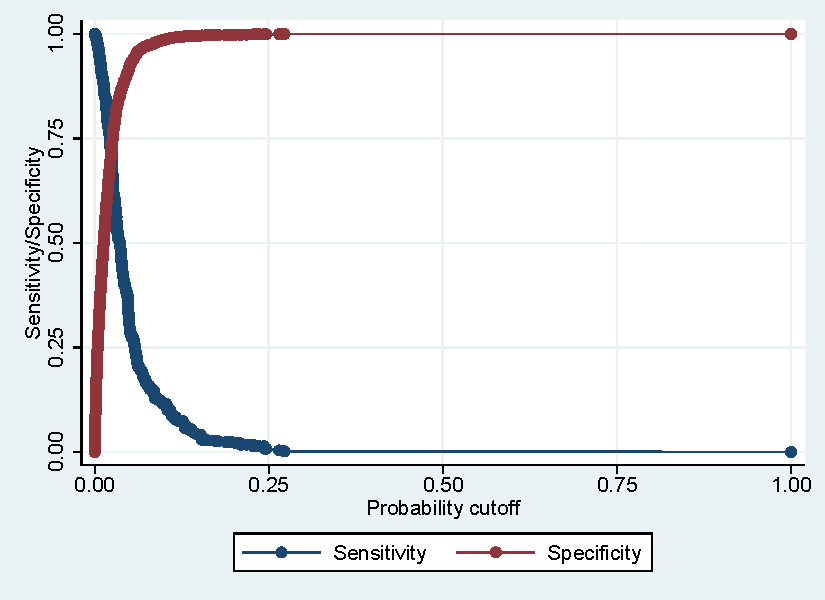
\includegraphics[width=0.7\textwidth]{book_37.pdf}
    \caption{The sensitivity-specificity curves.}
    \label{fig:sensspec}
\end{figure}

The gense(se) option tells Stata to generate a new variable called se, where the variable stores the values of sensitivity. The gensp(sp) option tells Stata to generate a new 
variable called sp, where the variable stores the values of specificity. Finally, the genp(cutp) option tells Stata to generate a new variable called cutp, where the variable 
stores the value of the cutoff point. The result of running the above command will be the generation of these new variables as well as the graph that is shown in Figure ~\ref{fig:sensspec}. 
We see that the sensitivity and the specificity curves intersect at a very small probability. To find the exact value of this probability we can generate a new variable that 
represents the difference between sensitivity and specificity, and then we can sort the dataset on this variable:

\begin{stlog}. gen diff = abs(se - sp)
(22,132 missing values generated)
{\smallskip}
. sort diff
{\smallskip}
\end{stlog}

Notice that we use the abs() function, which returns the absolute value. This is because we are not interested in the sign of the difference. We are interested in the smallest magnitude. 
Once we sort the observations on the new variable, the observation with the smallest value will appear at the very top. We display this observation using the following command:

\begin{stlog}. list sp se cutp diff in 1
{\smallskip}
     {\TLC}\HLI{43}{\TRC}
     {\VBAR}       sp         se       cutp       diff {\VBAR}
     {\LFTT}\HLI{43}{\RGTT}
  1. {\VBAR} 0.716377   0.716270   0.024088   .0001075 {\VBAR}
     {\BLC}\HLI{43}{\BRC}
{\smallskip}
\end{stlog}

We see that the cutoff p-value is 0.024088. We can now produce the classification table:

\begin{stlog}. estat class, cut(0.024088)
{\smallskip}
Logistic model for withdraw
{\smallskip}
              \HLI{8} True \HLI{8}
Classified {\VBAR}         D            {\tytilde}D  {\VBAR}      Total
\HLI{11}{\PLUS}\HLI{26}{\PLUS}\HLI{11}
     +     {\VBAR}       361          6973  {\VBAR}       7334
     -     {\VBAR}       143         17683  {\VBAR}      17826
\HLI{11}{\PLUS}\HLI{26}{\PLUS}\HLI{11}
   Total   {\VBAR}       504         24656  {\VBAR}      25160
{\smallskip}
Classified + if predicted Pr(D) >= .024088
True D defined as withdraw != 0
\HLI{50}
Sensitivity                     Pr( +| D)   71.63\%
Specificity                     Pr( -|{\tytilde}D)   71.72\%
Positive predictive value       Pr( D| +)    4.92\%
Negative predictive value       Pr({\tytilde}D| -)   99.20\%
\HLI{50}
False + rate for true {\tytilde}D        Pr( +|{\tytilde}D)   28.28\%
False - rate for true D         Pr( -| D)   28.37\%
False + rate for classified +   Pr({\tytilde}D| +)   95.08\%
False - rate for classified -   Pr( D| -)    0.80\%
\HLI{50}
Correctly classified                        71.72\%
\HLI{50}
{\smallskip}
\end{stlog}

We see that the model correctly classifies 71.72% of the observations, which is an acceptable value. 
\subsection{ROC Curve}
As discussed in the theory section, another way to test the model fit is to calculate the area under the ROC curve. To do that, we run the following command:

\begin{stlog}. lroc
{\smallskip}
Logistic model for withdraw
{\smallskip}
number of observations =    25160
area under ROC curve   =   0.7803
{\smallskip}
\end{stlog}
\begin{figure}[h]
    \centering
    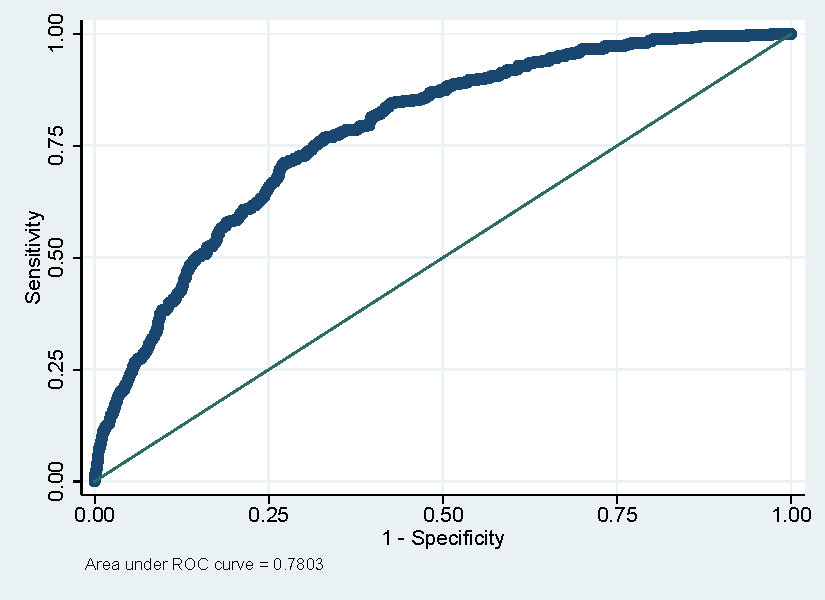
\includegraphics[width=0.7\textwidth]{book_41.pdf}
    \caption{The ROC curve.}
    \label{fig:roc}
\end{figure}

The resulting graph is shown in Figure ~\ref{fig:roc}. The output shows that the area under the curve is 0.7803. According to the set of rules that were mentioned in the theory section, this is considered acceptable 
discrimination.
\subsection{Residual Analysis}
When discussing the theory of logistic regression, it was mentioned that the three most commonly used ones are the standardized residuals, the deviance residuals, and the DeltaX residuals. 
We will now see how to calculate these in Stata.
\subsubsection{Standardized Residuals}
In order to calculate the standardized residuals in Stata, we use the following command right after we fit the model:

\begin{stlog}. predict residuals, rstandard
{\smallskip}
\end{stlog}

Since we want to plot the residuals against the predicted values, we will also need to calculate the predicted probabilities:

\begin{stlog}. predict prob
(option {\bftt{pr}} assumed; Pr(withdraw))
{\smallskip}
\end{stlog}

We can now plot the standardized residuals against the predicted probabilities:

\begin{stlog}. scatter residuals prob, yline(0) msize(vsmall)
{\smallskip}
\end{stlog}
\begin{figure}[h]
    \centering
    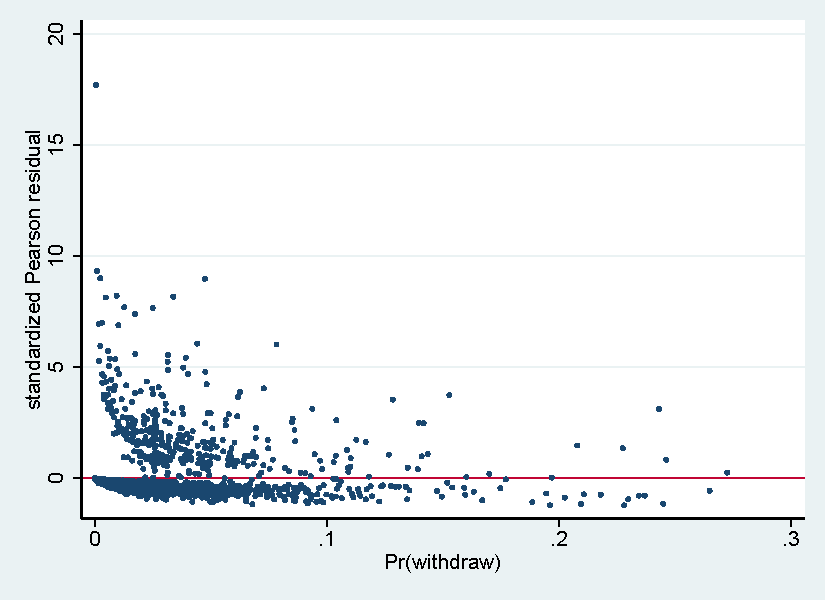
\includegraphics[width=0.7\textwidth]{book_44.pdf}
    \caption{Plotting the standardized residuals against the predicted probabilities.}
    \label{fig:res1}
\end{figure}

We use the yline(0) option in order to draw the line where y, which is the standardized residuals, are zero. This helps us visualize where the residuals are close to the value zero 
and where are they far from it. We also set the size of the dots to very small because there is a large number of observations. The graph is shown in Figure ~\ref{fig:res1}.

\subsubsection{Deviance Residuals} 
To calculate the deviance residuals, we use the command:

\begin{stlog}. predict dv, deviance
{\smallskip}
\end{stlog}

We then plot the statistic against the predicted probabilities, which we have already calculated:

\begin{stlog}. scatter dv prob, yline(2) msize(vsmall)
{\smallskip}
\end{stlog}
\begin{figure}[h]
    \centering
    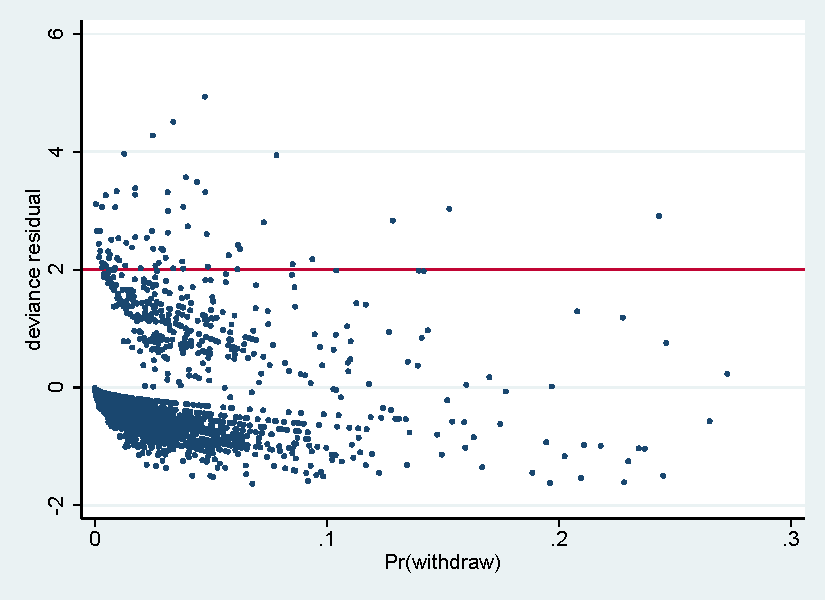
\includegraphics[width=0.7\textwidth]{book_46.pdf}
    \caption{Plotting the deviance residuals against the predicted probabilities (values above four are considered to be outliers).}
    \label{fig:res2}
\end{figure}

The graph is shown in Figure ~\ref{fig:res2}. Both Figure ~\ref{fig:res1} and Figure ~\ref{fig:res2} show that there are some observations that have residual values that are large when compared to other observations. 
In general, when the sample size is large enough, as is the case in our dataset, an observation that has a deviance residual that is greater than two should raise a flag, which is why we drew a horizontal 
line at the point y equal to two when plotting the deviance residuals.

\subsubsection{DeltaX}
To calculate the DeltaX residuals, we use the following command:

\begin{stlog}. predict dx2, dx2
{\smallskip}
\end{stlog}

We then produce the scatter plot against the predicted probabilities:

\begin{stlog}. scatter dx2 prob, yline(4) msize(vsmall)
{\smallskip}
\end{stlog}
\begin{figure}[h]
    \centering
    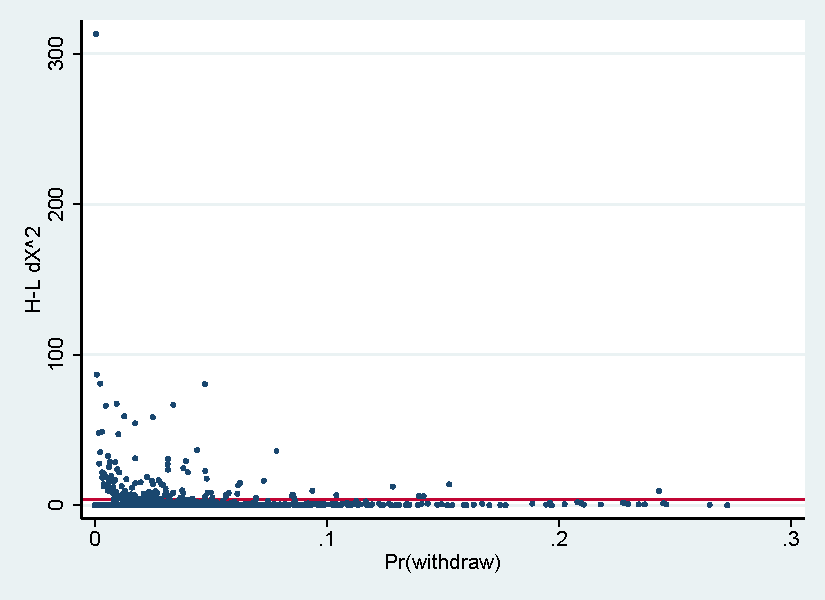
\includegraphics[width=0.7\textwidth]{book_48.pdf}
    \caption{Plotting the DeltaX residuals against the deviance residuals (values above four are considered to be outliers).}
    \label{fig:res3}
\end{figure}

We draw a horizontal line at the y equal 4 point since values above four are considered to be outliers. The output is shown in Figure ~\ref{fig:res3}.
\subsection{Influential Observations}
\subsubsection{The Hat Diagonal Statistic}
To calculate the hat statistic, we use the following command:

\begin{stlog}. predict hat, hat
{\smallskip}
\end{stlog}

We then plot the statistic against the predicted probability:

\begin{stlog}. scatter hat prob, yline(0.00519402) msize(vsmall)
{\smallskip}
\end{stlog}
\begin{figure}[h]
    \centering
    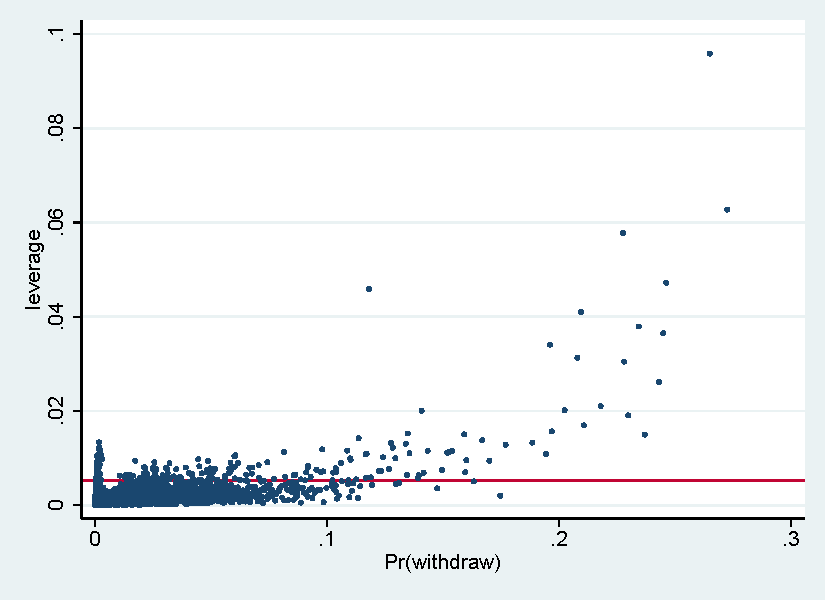
\includegraphics[width=0.7\textwidth]{book_50.pdf}
    \caption{Plotting the hat statistic residuals against the predicted probabilities (values that are more than two times greater than the average are considered to be influential).}
    \label{fig:influence1}
\end{figure}

We draw a horizontal line at the y equal 0.00519402 point since values that are more than two times greater than the average are considered to be influential (the mean of the variable hat is 0.002597). 
The graph is shown in Figure ~\ref{fig:influence1}. 
\subsubsection{Delta-Beta Statistic}
To calculate the delta-beta influence statistic, we use the following command:

\begin{stlog}. predict dbeta, dbeta
{\smallskip}
\end{stlog}

We then plot the values against the predicted probabilities:

\begin{stlog}. scatter dbeta prob, yline(1) msize(vsmall)
{\smallskip}
\end{stlog}
\begin{figure}[h]
    \centering
    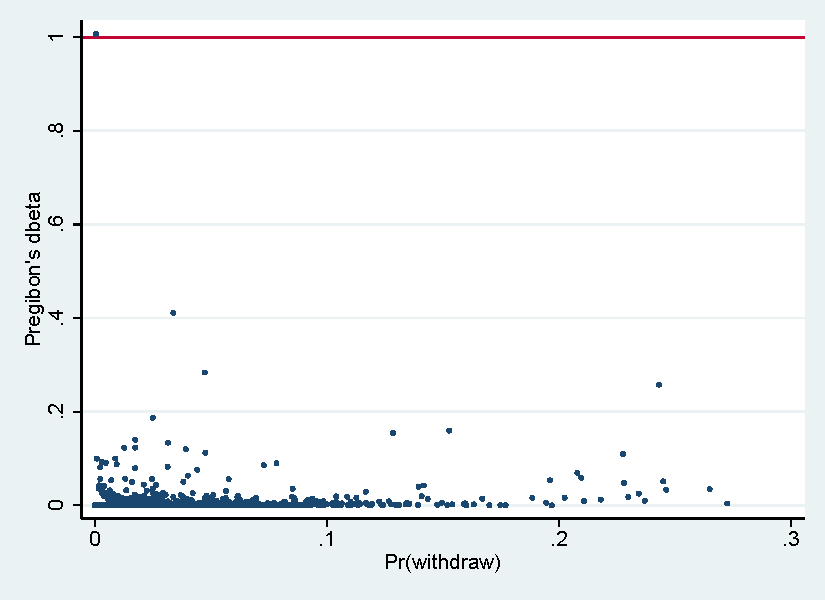
\includegraphics[width=0.7\textwidth]{book_52.pdf}
    \caption{Plotting the Delta-Beta statistic against the predicted probabilities.}
    \label{fig:influence2}
\end{figure}

We specify the yline(1) option because values greater than one indicate that the observation is influential. The graph is shown in Figure ~\ref{fig:influence2}.

So far, the graphs that have been produced have indicated that we have both outliers and influential observations. At this point it would be instructive to see how we can combine these two findings together. 
What we want is to produce a single graph that will include information about the size of the residuals (being an outlier) and the size of the leverage (having influence). Such a plot can be produced by using 
the following command:

\begin{stlog}. scatter dx2 prob [aweight=dbeta], msymbol(Oh)
{\smallskip}
\end{stlog}
\begin{figure}[h]
    \centering
    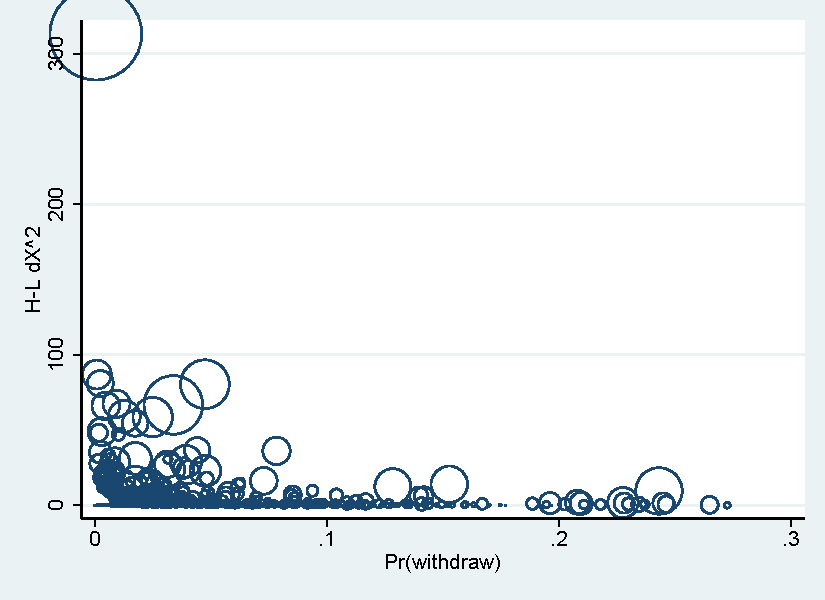
\includegraphics[width=0.7\textwidth]{book_53.pdf}
    \caption{Plot of DeltaX versus estimated probability weighted by the variable delta-beta.}
    \label{fig:influence3}
\end{figure}

What we are doing here is that we are producing a scatter plot of the DeltaX residuals against the predicted probabilities. We have actually already done this in Figure ~\ref{fig:res3}. This time however, 
the size of the dots are weighted by the value of the delta-beta statistic. Since DeltaX is a residual measure, the larger the value, the worse the fit of the observation, since residuals 
are a measure of the difference between the observed value and the predicted value. Since delta-measure is a measure of influence, and since we are weighing the dots by this variable, 
the larger the dot, the more influential it is. What this means is that when we produce this plot, the most problematic points are the large points in the upper left corner. 
This means that they are influential (hence their large size) and they are not a good fit with the model (high value of the residual which leads to them being near the top).

The graph produced by the above command in shown in Figure ~\ref{fig:influence3}. The large circle in the top left-hand side of the graph raises concerns. We need to take a closer look at these values. To do that, 
we ask Stata to list all observations that have a DeltaX residual that is greater than 200 (since we want to look at the circle in the top left-corner):

\begin{stlog}. list withdraw gender gpa college spring level3 if dx2 > 200, noobs
{\smallskip}
  {\TLC}\HLI{80}{\TRC}
  {\VBAR}    withdraw   gender    gpa       college           spring              level3 {\VBAR}
  {\LFTT}\HLI{80}{\RGTT}
  {\VBAR} No withdraw     male   79.3   Engineering   Fall or Summer   500 level courses {\VBAR}
  {\VBAR} No withdraw     male   79.3   Engineering   Fall or Summer   500 level courses {\VBAR}
  {\VBAR} No withdraw     male   79.3   Engineering   Fall or Summer   500 level courses {\VBAR}
  {\VBAR} No withdraw     male   79.3   Engineering   Fall or Summer   500 level courses {\VBAR}
  {\VBAR} No withdraw     male   79.3   Engineering   Fall or Summer   500 level courses {\VBAR}
  {\LFTT}\HLI{80}{\RGTT}
  {\VBAR}    Withdraw     male   79.3   Engineering   Fall or Summer   500 level courses {\VBAR}
  {\BLC}\HLI{80}{\BRC}
{\smallskip}
\end{stlog}

We see that there are six observations (the noobs option tells Stata not to list the observation numbers). We also notice that they all have a similar pattern: male engineering student with a GPA of 79.3, taking a 500-level course in a 
semester other than the spring semester. It seems that our model is not doing a good job of predicting the probability for observations with these covariate patterns. 
What would happen if we fit the model without including these observations? Let us see whether there will be a large change in the output:

\begin{stlog}. qui logistic withdraw gpa c.gpa\#c.gpa i.gender i.spring i.level3
{\smallskip}
. qui estimates store model1
{\smallskip}
. qui logistic withdraw gpa c.gpa\#c.gpa i.gender i.spring i.level3 if dx2 <= 200
{\smallskip}
. qui estimates store model2
{\smallskip}
. esttab model1 model2
{\smallskip}
\HLI{44}
                      (1)             (2)   
                 withdraw        withdraw   
\HLI{44}
withdraw                                    
gpa                 0.197*          0.200*  
                   (2.29)          (2.32)   
{\smallskip}
c.gpa\#c.gpa      -0.00231***     -0.00233***
                  (-3.73)         (-3.75)   
{\smallskip}
0.gender                0               0   
                      (.)             (.)   
{\smallskip}
1.gender            0.428***        0.425** 
                   (3.31)          (3.29)   
{\smallskip}
0.spring                0               0   
                      (.)             (.)   
{\smallskip}
1.spring            0.202*          0.206*  
                   (2.20)          (2.25)   
{\smallskip}
0.level3                0               0   
                      (.)             (.)   
{\smallskip}
1.level3            0.683***        0.682***
                   (7.19)          (7.18)   
{\smallskip}
2.level3           -2.617**             0   
                  (-2.61)             (.)   
{\smallskip}
_cons              -6.432*         -6.525*  
                  (-2.17)         (-2.20)   
\HLI{44}
N                   25160           24003   
\HLI{44}
t statistics in parentheses
* p<0.05, ** p<0.01, *** p<0.001
{\smallskip}
\end{stlog}

We first fit the model that included all observations and stored the results by using the estimates store command. These estimates were stored using the name model1. We then fit the model again, 
but this time we excluded the observations by including the if dx2 < 200 condition. This means that the six observations that have a DeltaX residual that is greater than 200 are excluded. We 
then stored the results under the name model2. Finally, we use the esttab command to print the results from both model1 and model2 (if the command is not installed on your computer, you can 
install the package in which it comes by running the command ssc install estout). We see that neither values of the coefficients, nor the significance levels of any of the variables changes significantly. 
This means that our results are robust.
\section{Interpreting the Results}
Now that we have seen that the model fit is good, it is time to interpret the obtained model parameters. As usual, Stata allows us to do this using both graphical tools and non-graphical tools. It 
is important to note that logistic regression has the following linear form:

$$ \log(\frac{p}{1-p})=ax+b $$

Therefore, once we fit the model we can calculate the value of the logit function for each observation. From this logit function, we are able to calculate the individual probabilities. Ultimately, we are interested 
in knowing the effect that each independent variable has on the probability of the event occurring. Does taking a course in the spring semester lead to an increase in the probability that a student might 
withdraw from the course? If so, what is the increase in the probability? Therefore, when we interpret the results, it is useful to know how the probability of the event occurring changes with changing values of the 
independent variables.
\subsection{Non-Graphical Interpretation}
There are several types of statistics that help us calculate the change in the probability relative to a change in the independent variable. Perhaps the most useful of these statistics is the discrete change, 
which is the change in probability given a change in the independent variable. To calculate discrete change in Stata, we will need to use the mchange command which is part of the SPost package. 
Therefore, you need to install the package in order to use the mchange command:

\begin{stlog}net from http://www.indiana.edu/{\tytilde}jslsoc/stata/
net install spost13_ado
\end{stlog}

Once you execute these commands, you can take advantage of the powerful tools that come with this package. To illustrate this, first fit the full logistic model:

\begin{stlog}. logistic withdraw gpa c.gpa\#c.gpa i.gender i.spring i.level3
{\smallskip}
Logistic regression                             Number of obs     =     25,160
                                                LR chi2(6)        =     539.84
                                                Prob > chi2       =     0.0000
Log likelihood = -2199.8567                     Pseudo R2         =     0.1093
{\smallskip}
\HLI{19}{\TOPT}\HLI{64}
          withdraw {\VBAR} Odds Ratio   Std. Err.      z    P>|z|     [95\% Conf. Interval]
\HLI{19}{\PLUS}\HLI{64}
               gpa {\VBAR}   1.217242   .1043142     2.29   0.022     1.029038    1.439868
                   {\VBAR}
       c.gpa\#c.gpa {\VBAR}   .9976954   .0006179    -3.73   0.000     .9964851    .9989072
                   {\VBAR}
            gender {\VBAR}
             male  {\VBAR}   1.534498   .1985629     3.31   0.001     1.190752    1.977476
                   {\VBAR}
            spring {\VBAR}
           Spring  {\VBAR}     1.2234    .111873     2.20   0.027     1.022659    1.463545
                   {\VBAR}
            level3 {\VBAR}
200 level courses  {\VBAR}     1.9789   .1879736     7.19   0.000     1.642741    2.383848
500 level courses  {\VBAR}   .0729881    .073254    -2.61   0.009     .0102082    .5218603
                   {\VBAR}
             _cons {\VBAR}   .0016093   .0047734    -2.17   0.030     4.81e-06     .538842
\HLI{19}{\BOTT}\HLI{64}
Note: _cons estimates baseline odds.
{\smallskip}
\end{stlog}

Next, we will use the mchange command in order to calculate the discrete change in the probability when GPA changes by 10:

\begin{stlog}. mchange gpa, delta(10)
{\smallskip}
logit: Changes in Pr(y) | Number of obs = 25160
{\smallskip}
Expression: Pr(withdraw), predict(pr)
{\smallskip}
             {\VBAR}    Change    p-value 
\HLI{13}{\PLUS}\HLI{22}
gpa          {\VBAR}                      
          +1 {\VBAR}    -0.002      0.000 
      +delta {\VBAR}    -0.015      0.000 
    Marginal {\VBAR}    -0.003      0.000 
{\smallskip}
Average predictions
{\smallskip}
             {\VBAR} No with{\tytilde}w   Withdraw 
\HLI{13}{\PLUS}\HLI{22}
  Pr(y|base) {\VBAR}     0.980      0.020 
{\smallskip}
1: Delta equals 10.
{\smallskip}
\end{stlog}

We use the delta(10) option in order to tell Stata that we want to calculate the change in probability when GPA changes by 10. This output shows that “on average, an increase in 10 points in the GPA decreases 
the probability of withdrawing from a course by 0.015.” As you can see, this is a clear interpretation. We are no longer talking about logit functions, odds, or even odds ratio. We are talking about the change 
in the probability that a certain event will happen. We can also use the option stat() in order to see exactly how the probability changes:

\begin{stlog}. mchange gpa, delta(10) stat(change from to pvalue)
{\smallskip}
logit: Changes in Pr(y) | Number of obs = 25160
{\smallskip}
Expression: Pr(withdraw), predict(pr)
{\smallskip}
             {\VBAR}    Change       From         To    p-value 
\HLI{13}{\PLUS}\HLI{44}
gpa          {\VBAR}                                            
          +1 {\VBAR}    -0.002      0.020      0.018      0.000 
      +delta {\VBAR}    -0.015      0.020      0.005      0.000 
    Marginal {\VBAR}    -0.003         .z         .z      0.000 
{\smallskip}
Average predictions
{\smallskip}
             {\VBAR} No with{\tytilde}w   Withdraw 
\HLI{13}{\PLUS}\HLI{22}
  Pr(y|base) {\VBAR}     0.980      0.020 
{\smallskip}
1: Delta equals 10.
{\smallskip}
\end{stlog}

We specified the stat() option in order to tell Stata that we want to see the change in probability, the value from which the probability changed, the value to which the probability changes when GPA increases by 10, 
and the p-value of the result. We see that, on average, the probability changes from 0.02 to 0.005 when GPA changes by 10. This is a decrease of 0.015. 

We can also use the mchange command when the independent variable is binary:

\begin{stlog}. mchange gender, stat(change from to pvalue)
{\smallskip}
logit: Changes in Pr(y) | Number of obs = 25160
{\smallskip}
Expression: Pr(withdraw), predict(pr)
{\smallskip}
                {\VBAR}    Change       From         To    p-value 
\HLI{16}{\PLUS}\HLI{44}
gender          {\VBAR}                                            
 male vs female {\VBAR}     0.007      0.014      0.022      0.000 
{\smallskip}
Average predictions
{\smallskip}
             {\VBAR} No with{\tytilde}w   Withdraw 
\HLI{13}{\PLUS}\HLI{22}
  Pr(y|base) {\VBAR}     0.980      0.020 
{\smallskip}
{\smallskip}
\end{stlog}

Notice that we did not specify the delta() option. This is because the only meaningful change in the variable gender is from zero to one, given that the variable is binary. The result shows that 
“on average, being a male increases the probability of course withdrawal from 0.014 to 0.022, which is a change of 0.007 (p $<$ 0.05).” 

The command can also be used when the independent variable has more than two categories:

\begin{stlog}. mchange level3, stat(change from to pvalue)
{\smallskip}
logit: Changes in Pr(y) | Number of obs = 25160
{\smallskip}
Expression: Pr(withdraw), predict(pr)
{\smallskip}
                                 {\VBAR}    Change       From         To    p-value 
\HLI{33}{\PLUS}\HLI{44}
level3                           {\VBAR}                                            
 200 level courses vs Other co{\tytilde}s {\VBAR}     0.013      0.014      0.028      0.000 
 500 level courses vs Other co{\tytilde}s {\VBAR}    -0.013      0.014      0.001      0.000 
 500 level courses vs 200 leve{\tytilde}c {\VBAR}    -0.027      0.028      0.001      0.000 
{\smallskip}
Average predictions
{\smallskip}
             {\VBAR} No with{\tytilde}w   Withdraw 
\HLI{13}{\PLUS}\HLI{22}
  Pr(y|base) {\VBAR}     0.980      0.020 
{\smallskip}
{\smallskip}
\end{stlog}

Here, we are looking at the change in probability depending on the level of the course. The output of the command is shown in Figure 49. The result indicates that, “on average, taking a 
200-level course compared to taking courses classified as ‘other’ increases the probability of course withdrawal by 0.013 (p $<$ 0.05). Taking a 500-level course compared to taking courses 
classified as ‘other’ decreases the probability of course withdrawal by 0.013 (p $<$ 0.05). Taking a 500-level course compared to taking a 200-level course decreases the probability of course withdrawal 
by 0.027 (p $<$ 0.05).”

\subsection{Graphical Interpretation}
As we saw in the previous section, interpreting the results in terms of the calculated probability is very intuitive and clear. In addition to calculating the discrete changes, it is also very useful if we can 
produce graphs that summarize the results. As an example, take the case of the independent GPA. We would like to know what is the change in the probability of withdrawing from a course when GPA changes. 
We use the margins command to tell Stata to calculate the probabilities of withdrawal at different values of GPA:

\begin{stlog}. margins, at(gpa=(40(1)100)) noatlegend
{\smallskip}
Predictive margins                              Number of obs     =     25,160
Model VCE    : OIM
{\smallskip}
Expression   : Pr(withdraw), predict()
{\smallskip}
\HLI{13}{\TOPT}\HLI{64}
             {\VBAR}            Delta-method
             {\VBAR}     Margin   Std. Err.      z    P>|z|     [95\% Conf. Interval]
\HLI{13}{\PLUS}\HLI{64}
         _at {\VBAR}
          1  {\VBAR}   .1696368    .074682     2.27   0.023     .0232628    .3160107
          2  {\VBAR}   .1709642   .0703718     2.43   0.015      .033038    .3088904
          3  {\VBAR}   .1716635   .0659951     2.60   0.009     .0423155    .3010115
          4  {\VBAR}   .1717288   .0615925     2.79   0.005     .0510097     .292448
          5  {\VBAR}   .1711597   .0572023     2.99   0.003     .0590452    .2832741
          6  {\VBAR}   .1699608   .0528601     3.22   0.001     .0663569    .2735646
          7  {\VBAR}   .1681423   .0485987     3.46   0.001     .0728906     .263394
          8  {\VBAR}   .1657199   .0444483     3.73   0.000     .0786028    .2528371
          9  {\VBAR}   .1627143   .0404363     4.02   0.000     .0834606     .241968
         10  {\VBAR}   .1591515    .036587     4.35   0.000     .0874422    .2308607
         11  {\VBAR}   .1550624   .0329219     4.71   0.000     .0905366    .2195882
         12  {\VBAR}   .1504829   .0294595     5.11   0.000     .0927433    .2082224
         13  {\VBAR}   .1454533   .0262149     5.55   0.000     .0940731    .1968335
         14  {\VBAR}   .1400183      .0232     6.04   0.000     .0945472    .1854894
         15  {\VBAR}   .1342264   .0204232     6.57   0.000     .0941977    .1742551
         16  {\VBAR}   .1281292   .0178892     7.16   0.000      .093067    .1631914
         17  {\VBAR}   .1217811   .0155989     7.81   0.000     .0912079    .1523544
         18  {\VBAR}   .1152385   .0135491     8.51   0.000     .0886828    .1417943
         19  {\VBAR}    .108559   .0117327     9.25   0.000     .0855634    .1315547
         20  {\VBAR}   .1018004   .0101384    10.04   0.000     .0819296    .1216713
         21  {\VBAR}     .09502   .0087511    10.86   0.000     .0778681    .1121719
         22  {\VBAR}   .0882735   .0075526    11.69   0.000     .0734707    .1030764
         23  {\VBAR}   .0816143    .006522    12.51   0.000     .0688314    .0943973
         24  {\VBAR}   .0750924   .0056372    13.32   0.000     .0640438    .0861411
         25  {\VBAR}   .0687535    .004876    14.10   0.000     .0591968    .0783103
         26  {\VBAR}   .0626387   .0042178    14.85   0.000     .0543719    .0709056
         27  {\VBAR}   .0567835   .0036448    15.58   0.000     .0496398    .0639273
         28  {\VBAR}   .0512177   .0031425    16.30   0.000     .0450585    .0573769
         29  {\VBAR}   .0459647   .0027002    17.02   0.000     .0406724    .0512571
         30  {\VBAR}   .0410421   .0023109    17.76   0.000     .0365128    .0455715
         31  {\VBAR}   .0364613   .0019706    18.50   0.000     .0325989    .0403237
         32  {\VBAR}   .0322279   .0016777    19.21   0.000     .0289396    .0355162
         33  {\VBAR}    .028342   .0014319    19.79   0.000     .0255354    .0311485
         34  {\VBAR}   .0247988   .0012332    20.11   0.000     .0223817    .0272159
         35  {\VBAR}   .0215895   .0010806    19.98   0.000     .0194716    .0237074
         36  {\VBAR}   .0187013   .0009702    19.28   0.000     .0167997     .020603
         37  {\VBAR}   .0161187   .0008953    18.00   0.000     .0143641    .0178734
         38  {\VBAR}   .0138238   .0008461    16.34   0.000     .0121654    .0154822
         39  {\VBAR}   .0117971   .0008129    14.51   0.000      .010204    .0133903
         40  {\VBAR}   .0100181   .0007868    12.73   0.000      .008476    .0115602
         41  {\VBAR}   .0084658   .0007619    11.11   0.000     .0069726    .0099591
         42  {\VBAR}   .0071193   .0007343     9.70   0.000     .0056802    .0085585
         43  {\VBAR}   .0059581   .0007022     8.48   0.000     .0045817    .0073344
         44  {\VBAR}   .0049622   .0006654     7.46   0.000     .0036581    .0062663
         45  {\VBAR}   .0041131   .0006241     6.59   0.000     .0028898    .0053364
         46  {\VBAR}    .003393   .0005795     5.86   0.000     .0022573    .0045287
         47  {\VBAR}   .0027858   .0005325     5.23   0.000      .001742    .0038295
         48  {\VBAR}   .0022764   .0004845     4.70   0.000     .0013267    .0032261
         49  {\VBAR}   .0018514   .0004367     4.24   0.000     .0009955    .0027072
         50  {\VBAR}   .0014986   .0003899     3.84   0.000     .0007346    .0022627
         51  {\VBAR}   .0012075    .000345     3.50   0.000     .0005314    .0018835
         52  {\VBAR}   .0009683   .0003026     3.20   0.001     .0003752    .0015614
         53  {\VBAR}   .0007729   .0002632     2.94   0.003      .000257    .0012888
         54  {\VBAR}   .0006141   .0002271     2.70   0.007     .0001689    .0010592
         55  {\VBAR}   .0004856   .0001944     2.50   0.013     .0001045    .0008667
         56  {\VBAR}   .0003822   .0001652     2.31   0.021     .0000584     .000706
         57  {\VBAR}   .0002995   .0001393     2.15   0.032     .0000264    .0005726
         58  {\VBAR}   .0002336   .0001167     2.00   0.045     4.88e-06    .0004622
         59  {\VBAR}   .0001813    .000097     1.87   0.062    -8.83e-06    .0003714
         60  {\VBAR}   .0001401   .0000801     1.75   0.080    -.0000169    .0002971
         61  {\VBAR}   .0001077   .0000657     1.64   0.101     -.000021    .0002365
\HLI{13}{\BOTT}\HLI{64}
{\smallskip}
\end{stlog}

We have already used this command when we were visualizing the effect of including a quadratic term. There are two differences. The first difference is that the logistic model includes other independent variables as well. 
The second difference is that we do not use the predict(xb) option. This is a very important point. We previously specified this option because we want to calculate the value of the logit function $\log(\frac{p}{1-p})$, 
since we were testing for linearity. What we now want to do is to calculate the value of p, the probability. By default, margins calculates probability. As we said, when visualizing the results, we are more 
interested in seeing the effect of the independent variables on the probability of the event occurring. Figure 50 shows part of the output produced when we run the command.

We have already used this command when we were visualizing the effect of including a quadratic term. There are two differences. The first difference is that the logistic model includes other independent variables as 
well. The second difference is that we do not use the predict(xb) option. This is a very important point. We previously specified this option because we want to calculate the value 
of the logit function $\log(\frac{p}{1-p})$, since we were testing for linearity. What we now want to do is to calculate the value of p, the probability. By default, margins calculates 
probability. As we said, when visualizing the results, we are more interested in seeing the effect of the independent variables on the probability of the event occurring. 
Figure 50 shows part of the output produced when we run the command.

We can tell Stata to plot these results using the marginsplot command:

\begin{stlog}. marginsplot, noci
{\smallskip}
  Variables that uniquely identify margins: gpa
{\smallskip}
\end{stlog}
\begin{figure}[h]
    \centering
    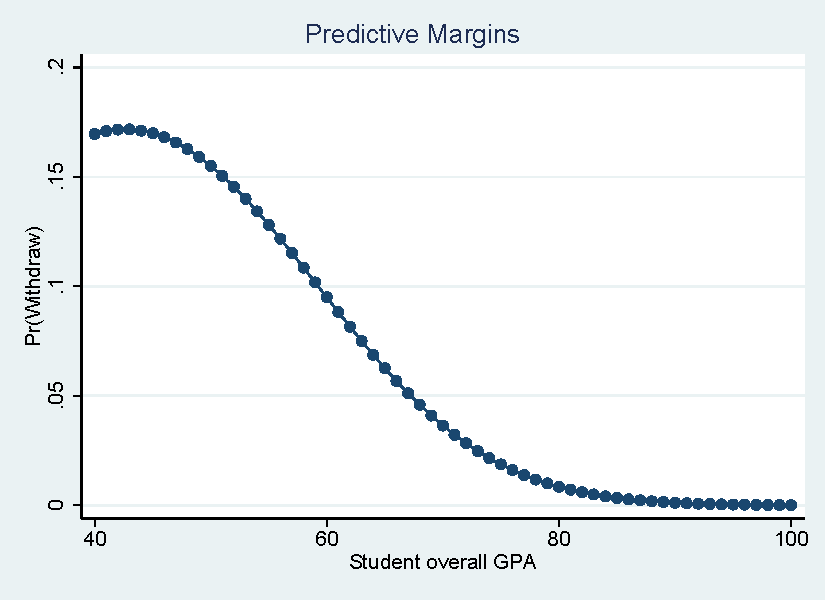
\includegraphics[width=0.7\textwidth]{book_63.pdf}
    \caption{Graphing the probability of withdrawing from a course for each value of GPA.}
    \label{fig:visual1}
\end{figure}

The graph is shown in Figure ~\ref{fig:visual1}. Notice that the probability drops to almost zero for values of GPA that are higher than 80.

We can also produce a more informative graph by including one of the categorical variables in the margins command:

\begin{stlog}. margins, at(gpa=(40(1)100) level3=(0 1 2)) noatlegend
{\smallskip}
Predictive margins                              Number of obs     =     25,160
Model VCE    : OIM
{\smallskip}
Expression   : Pr(withdraw), predict()
{\smallskip}
\HLI{13}{\TOPT}\HLI{64}
             {\VBAR}            Delta-method
             {\VBAR}     Margin   Std. Err.      z    P>|z|     [95\% Conf. Interval]
\HLI{13}{\PLUS}\HLI{64}
         _at {\VBAR}
          1  {\VBAR}   .1342941    .064038     2.10   0.036      .008782    .2598062
          2  {\VBAR}   .2340575   .0970792     2.41   0.016     .0437857    .4243292
          3  {\VBAR}   .0112565   .0127349     0.88   0.377    -.0137034    .0362164
          4  {\VBAR}   .1354203   .0604817     2.24   0.025     .0168783    .2539623
          5  {\VBAR}   .2357871   .0913759     2.58   0.010     .0566936    .4148807
          6  {\VBAR}    .011365   .0126729     0.90   0.370    -.0134734    .0362033
          7  {\VBAR}   .1360141   .0568347     2.39   0.017     .0246201    .2474081
          8  {\VBAR}   .2366977   .0856353     2.76   0.006     .0688556    .4045399
          9  {\VBAR}   .0114223   .0125675     0.91   0.363    -.0132097    .0360542
         10  {\VBAR}   .1360696   .0531367     2.56   0.010     .0319237    .2402155
         11  {\VBAR}   .2367828   .0799035     2.96   0.003     .0801748    .3933908
         12  {\VBAR}   .0114276   .0124199     0.92   0.358    -.0129149    .0357702
         13  {\VBAR}   .1355863   .0494255     2.74   0.006      .038714    .2324585
         14  {\VBAR}   .2360417   .0742229     3.18   0.001     .0905674     .381516
         15  {\VBAR}    .011381   .0122313     0.93   0.352    -.0125918    .0353538
         16  {\VBAR}   .1345689   .0457371     2.94   0.003     .0449257     .224212
         17  {\VBAR}   .2344798   .0686324     3.42   0.001     .0999627    .3689969
         18  {\VBAR}   .0112829   .0120032     0.94   0.347     -.012243    .0348088
         19  {\VBAR}   .1330276    .042105     3.16   0.002     .0505033    .2155519
         20  {\VBAR}   .2321082   .0631675     3.67   0.000     .1083022    .3559143
         21  {\VBAR}   .0111348   .0117377     0.95   0.343    -.0118707    .0341404
         22  {\VBAR}   .1309778   .0385599     3.40   0.001     .0554018    .2065538
         23  {\VBAR}   .2289444   .0578604     3.96   0.000     .1155401    .3423487
         24  {\VBAR}   .0109387    .011437     0.96   0.339    -.0114775    .0333548
         25  {\VBAR}   .1284399   .0351297     3.66   0.000      .059587    .1972928
         26  {\VBAR}   .2250115   .0527403     4.27   0.000     .1216423    .3283806
         27  {\VBAR}    .010697   .0111035     0.96   0.335    -.0110655    .0324594
         28  {\VBAR}   .1254393   .0318391     3.94   0.000     .0630358    .1878428
         29  {\VBAR}   .2203389   .0478335     4.61   0.000     .1265868    .3140909
         30  {\VBAR}   .0104129     .01074     0.97   0.332    -.0106371    .0314629
         31  {\VBAR}   .1220058   .0287096     4.25   0.000      .065736    .1782757
         32  {\VBAR}    .214962   .0431634     4.98   0.000     .1303632    .2995608
         33  {\VBAR}   .0100902   .0103494     0.97   0.330    -.0101944    .0303747
         34  {\VBAR}   .1181737   .0257592     4.59   0.000     .0676866    .1686609
         35  {\VBAR}   .2089224   .0387505     5.39   0.000     .1329729     .284872
         36  {\VBAR}   .0097328   .0099351     0.98   0.327    -.0097397    .0292052
         37  {\VBAR}   .1139811   .0230022     4.96   0.000     .0688977    .1590646
         38  {\VBAR}   .2022676    .034612     5.84   0.000     .1344293    .2701058
         39  {\VBAR}   .0093451   .0095004     0.98   0.325    -.0092753    .0279655
         40  {\VBAR}   .1094694   .0204489     5.35   0.000     .0693902    .1495486
         41  {\VBAR}   .1950507   .0307621     6.34   0.000      .134758    .2553434
         42  {\VBAR}   .0089318   .0090489     0.99   0.324    -.0088037    .0266673
         43  {\VBAR}    .104683    .018106     5.78   0.000     .0691959    .1401701
         44  {\VBAR}   .1873306   .0272115     6.88   0.000     .1339971    .2406641
         45  {\VBAR}   .0084977   .0085842     0.99   0.322    -.0083271    .0253224
         46  {\VBAR}   .0996684   .0159758     6.24   0.000     .0683564    .1309804
         47  {\VBAR}    .179171   .0239665     7.48   0.000     .1321975    .2261445
         48  {\VBAR}   .0080475   .0081102     0.99   0.321    -.0078482    .0239433
         49  {\VBAR}   .0944738   .0140567     6.72   0.000     .0669232    .1220243
         50  {\VBAR}   .1706401   .0210295     8.11   0.000     .1294231    .2118572
         51  {\VBAR}   .0075863   .0076306     0.99   0.320    -.0073695     .022542
         52  {\VBAR}    .089148   .0123429     7.22   0.000     .0649564    .1133395
         53  {\VBAR}     .16181   .0183977     8.80   0.000     .1257511    .1978689
         54  {\VBAR}   .0071185   .0071492     1.00   0.319    -.0068936    .0211307
         55  {\VBAR}     .08374   .0108249     7.74   0.000     .0625237    .1049564
         56  {\VBAR}   .1527554   .0160633     9.51   0.000     .1212719    .1842389
         57  {\VBAR}   .0066489   .0066695     1.00   0.319    -.0064231     .019721
         58  {\VBAR}   .0782983   .0094897     8.25   0.000     .0596988    .0968977
         59  {\VBAR}   .1435528   .0140128    10.24   0.000     .1160882    .1710174
         60  {\VBAR}   .0061817   .0061951     1.00   0.318    -.0059606    .0183239
         61  {\VBAR}   .0728695   .0083214     8.76   0.000     .0565598    .0891792
         62  {\VBAR}   .1342793   .0122274    10.98   0.000      .110314    .1582445
         63  {\VBAR}   .0057208   .0057293     1.00   0.318    -.0055084      .01695
         64  {\VBAR}   .0674982   .0073023     9.24   0.000      .053186    .0818104
         65  {\VBAR}   .1250113   .0106834    11.70   0.000     .1040723    .1459503
         66  {\VBAR}   .0052698    .005275     1.00   0.318     -.005069    .0156086
         67  {\VBAR}   .0622261   .0064135     9.70   0.000     .0496558    .0747963
         68  {\VBAR}   .1158232   .0093531    12.38   0.000     .0974915     .134155
         69  {\VBAR}    .004832    .004835     1.00   0.318    -.0046445    .0143084
         70  {\VBAR}   .0570911   .0056365    10.13   0.000     .0460439    .0681384
         71  {\VBAR}    .106786    .008207    13.01   0.000     .0907006    .1228714
         72  {\VBAR}     .00441   .0044118     1.00   0.318    -.0042369    .0130569
         73  {\VBAR}   .0521274   .0049539    10.52   0.000     .0424179     .061837
         74  {\VBAR}    .097966   .0072153    13.58   0.000     .0838242    .1121078
         75  {\VBAR}   .0040063   .0040073     1.00   0.317    -.0038478    .0118604
         76  {\VBAR}   .0473644   .0043508    10.89   0.000     .0388371    .0558918
         77  {\VBAR}   .0894237   .0063507    14.08   0.000     .0769767    .1018708
         78  {\VBAR}   .0036227   .0036232     1.00   0.317    -.0034786    .0107241
         79  {\VBAR}   .0428269   .0038145    11.23   0.000     .0353507    .0503032
         80  {\VBAR}   .0812128   .0055894    14.53   0.000     .0702578    .0921678
         81  {\VBAR}   .0032607   .0032609     1.00   0.317    -.0031306     .009652
         82  {\VBAR}   .0385347   .0033354    11.55   0.000     .0319975    .0450719
         83  {\VBAR}   .0733792    .004913    14.94   0.000     .0637498    .0830086
         84  {\VBAR}   .0029213   .0029213     1.00   0.317    -.0028044     .008647
         85  {\VBAR}   .0345027   .0029065    11.87   0.000     .0288061    .0401992
         86  {\VBAR}   .0659607   .0043084    15.31   0.000     .0575164     .074405
         87  {\VBAR}   .0026051    .002605     1.00   0.317    -.0025005    .0077108
         88  {\VBAR}   .0307408    .002523    12.18   0.000     .0257959    .0356857
         89  {\VBAR}   .0589864   .0037671    15.66   0.000      .051603    .0663699
         90  {\VBAR}   .0023124   .0023122     1.00   0.317    -.0022193    .0068441
         91  {\VBAR}   .0272545   .0021819    12.49   0.000     .0229781     .031531
         92  {\VBAR}    .052477    .003285    15.97   0.000     .0460386    .0589154
         93  {\VBAR}   .0020431   .0020427     1.00   0.317    -.0019606    .0060467
         94  {\VBAR}    .024045   .0018814    12.78   0.000     .0203575    .0277324
         95  {\VBAR}   .0464446   .0028603    16.24   0.000     .0408385    .0520507
         96  {\VBAR}   .0017968   .0017963     1.00   0.317     -.001724    .0053175
         97  {\VBAR}   .0211093   .0016202    13.03   0.000     .0179339    .0242848
         98  {\VBAR}   .0408933   .0024931    16.40   0.000     .0360069    .0457797
         99  {\VBAR}   .0015728   .0015724     1.00   0.317     -.001509    .0046546
        100  {\VBAR}   .0184414   .0013971    13.20   0.000     .0157031    .0211796
        101  {\VBAR}   .0358201   .0021833    16.41   0.000     .0315409    .0400993
        102  {\VBAR}   .0013704     .00137     1.00   0.317    -.0013147    .0040556
        103  {\VBAR}   .0160319   .0012105    13.24   0.000     .0136593    .0184045
        104  {\VBAR}   .0312151   .0019296    16.18   0.000     .0274333     .034997
        105  {\VBAR}   .0011886   .0011882     1.00   0.317    -.0011402    .0035174
        106  {\VBAR}   .0138694   .0010581    13.11   0.000     .0117955    .0159433
        107  {\VBAR}   .0270632   .0017282    15.66   0.000      .023676    .0304504
        108  {\VBAR}   .0010261   .0010258     1.00   0.317    -.0009845    .0030366
        109  {\VBAR}   .0119403   .0009362    12.75   0.000     .0101054    .0137753
        110  {\VBAR}   .0233443   .0015725    14.85   0.000     .0202623    .0264264
        111  {\VBAR}   .0008817   .0008816     1.00   0.317    -.0008462    .0026096
        112  {\VBAR}   .0102299   .0008402    12.18   0.000     .0085831    .0118767
        113  {\VBAR}   .0200347   .0014533    13.79   0.000     .0171862    .0228832
        114  {\VBAR}   .0007541   .0007542     1.00   0.317    -.0007242    .0022324
        115  {\VBAR}   .0087222   .0007646    11.41   0.000     .0072235    .0102208
        116  {\VBAR}    .017108   .0013604    12.58   0.000     .0144417    .0197744
        117  {\VBAR}    .000642   .0006424     1.00   0.318    -.0006171    .0019011
        118  {\VBAR}    .007401   .0007039    10.51   0.000     .0060213    .0087806
        119  {\VBAR}    .014536   .0012839    11.32   0.000     .0120196    .0170524
        120  {\VBAR}   .0005441   .0005447     1.00   0.318    -.0005236    .0016117
        121  {\VBAR}   .0062499    .000653     9.57   0.000       .00497    .0075298
        122  {\VBAR}   .0122895   .0012157    10.11   0.000     .0099067    .0146723
        123  {\VBAR}   .0004589   .0004599     1.00   0.318    -.0004424    .0013603
        124  {\VBAR}   .0052527    .000608     8.64   0.000      .004061    .0064443
        125  {\VBAR}   .0103391   .0011502     8.99   0.000     .0080847    .0125935
        126  {\VBAR}   .0003853   .0003866     1.00   0.319    -.0003723     .001143
        127  {\VBAR}   .0043936    .000566     7.76   0.000     .0032843    .0055029
        128  {\VBAR}   .0086557   .0010839     7.99   0.000     .0065312    .0107801
        129  {\VBAR}   .0003221   .0003236     1.00   0.320    -.0003121    .0009562
        130  {\VBAR}   .0036576   .0005253     6.96   0.000     .0026281    .0046872
        131  {\VBAR}   .0072112   .0010152     7.10   0.000     .0052215    .0092009
        132  {\VBAR}   .0002679   .0002697     0.99   0.320    -.0002607    .0007965
        133  {\VBAR}   .0030306    .000485     6.25   0.000     .0020799    .0039813
        134  {\VBAR}   .0059787   .0009437     6.34   0.000     .0041292    .0078283
        135  {\VBAR}   .0002218   .0002238     0.99   0.322    -.0002169    .0006606
        136  {\VBAR}   .0024992    .000445     5.62   0.000     .0016271    .0033714
        137  {\VBAR}   .0049331   .0008699     5.67   0.000     .0032281    .0066382
        138  {\VBAR}   .0001829    .000185     0.99   0.323    -.0001798    .0005455
        139  {\VBAR}   .0020514   .0004052     5.06   0.000     .0012572    .0028456
        140  {\VBAR}    .004051   .0007951     5.10   0.000     .0024926    .0056093
        141  {\VBAR}     .00015   .0001523     0.98   0.325    -.0001485    .0004486
        142  {\VBAR}   .0016759   .0003661     4.58   0.000     .0009583    .0023935
        143  {\VBAR}   .0033107   .0007203     4.60   0.000      .001899    .0047225
        144  {\VBAR}   .0001225   .0001249     0.98   0.327    -.0001223    .0003673
        145  {\VBAR}   .0013627   .0003282     4.15   0.000     .0007195     .002006
        146  {\VBAR}    .002693   .0006469     4.16   0.000     .0014252    .0039608
        147  {\VBAR}   .0000996    .000102     0.98   0.329    -.0001004    .0002995
        148  {\VBAR}   .0011029   .0002918     3.78   0.000     .0005311    .0016748
        149  {\VBAR}   .0021801   .0005759     3.79   0.000     .0010514    .0033089
        150  {\VBAR}   .0000806    .000083     0.97   0.332    -.0000821    .0002433
        151  {\VBAR}   .0008885   .0002573     3.45   0.001     .0003842    .0013929
        152  {\VBAR}   .0017567   .0005084     3.46   0.001     .0007602    .0027532
        153  {\VBAR}   .0000649   .0000673     0.96   0.335     -.000067    .0001968
        154  {\VBAR}   .0007125   .0002251     3.16   0.002     .0002712    .0011537
        155  {\VBAR}   .0014089   .0004452     3.16   0.002     .0005363    .0022814
        156  {\VBAR}    .000052   .0000543     0.96   0.338    -.0000544    .0001585
        157  {\VBAR}   .0005686   .0001954     2.91   0.004     .0001856    .0009517
        158  {\VBAR}   .0011246   .0003867     2.91   0.004     .0003668    .0018825
        159  {\VBAR}   .0000415   .0000437     0.95   0.342    -.0000441    .0001272
        160  {\VBAR}   .0004517   .0001684     2.68   0.007     .0001218    .0007817
        161  {\VBAR}   .0008935   .0003332     2.68   0.007     .0002404    .0015467
        162  {\VBAR}    .000033    .000035     0.94   0.346    -.0000357    .0001017
        163  {\VBAR}   .0003572    .000144     2.48   0.013     .0000751    .0006394
        164  {\VBAR}   .0007066    .000285     2.48   0.013     .0001481    .0012652
        165  {\VBAR}   .0000261    .000028     0.93   0.351    -.0000288    .0000809
        166  {\VBAR}   .0002812   .0001222     2.30   0.021     .0000417    .0005206
        167  {\VBAR}   .0005562   .0002419     2.30   0.021     .0000821    .0010304
        168  {\VBAR}   .0000205   .0000223     0.92   0.357    -.0000231    .0000642
        169  {\VBAR}   .0002203    .000103     2.14   0.032     .0000185    .0004221
        170  {\VBAR}   .0004358   .0002039     2.14   0.033     .0000362    .0008354
        171  {\VBAR}   .0000161   .0000177     0.91   0.363    -.0000185    .0000507
        172  {\VBAR}   .0001718   .0000861     1.99   0.046     2.95e-06    .0003406
        173  {\VBAR}   .0003399   .0001706     1.99   0.046     5.50e-06    .0006743
        174  {\VBAR}   .0000125    .000014     0.90   0.369    -.0000148    .0000399
        175  {\VBAR}   .0001334   .0000716     1.86   0.062    -6.95e-06    .0002737
        176  {\VBAR}   .0002639   .0001418     1.86   0.063     -.000014    .0005417
        177  {\VBAR}   9.73e-06    .000011     0.89   0.376    -.0000118    .0000313
        178  {\VBAR}    .000103   .0000591     1.74   0.081    -.0000128    .0002188
        179  {\VBAR}   .0002039    .000117     1.74   0.081    -.0000255    .0004332
        180  {\VBAR}   7.52e-06   8.63e-06     0.87   0.383    -9.39e-06    .0000244
        181  {\VBAR}   .0000792   .0000484     1.64   0.102    -.0000157    .0001742
        182  {\VBAR}   .0001568   .0000959     1.63   0.102    -.0000312    .0003449
        183  {\VBAR}   5.78e-06   6.75e-06     0.86   0.391    -7.44e-06     .000019
\HLI{13}{\BOTT}\HLI{64}
{\smallskip}
\end{stlog}

In this case, we are telling Stata to calculate the probabilities when GPA ranges from 40 to 100 for each value of the categorical variable level3. We can then plot the graph:

\begin{stlog}. marginsplot, noci
{\smallskip}
  Variables that uniquely identify margins: gpa level3
{\smallskip}
\end{stlog}
\begin{figure}[h]
    \centering
    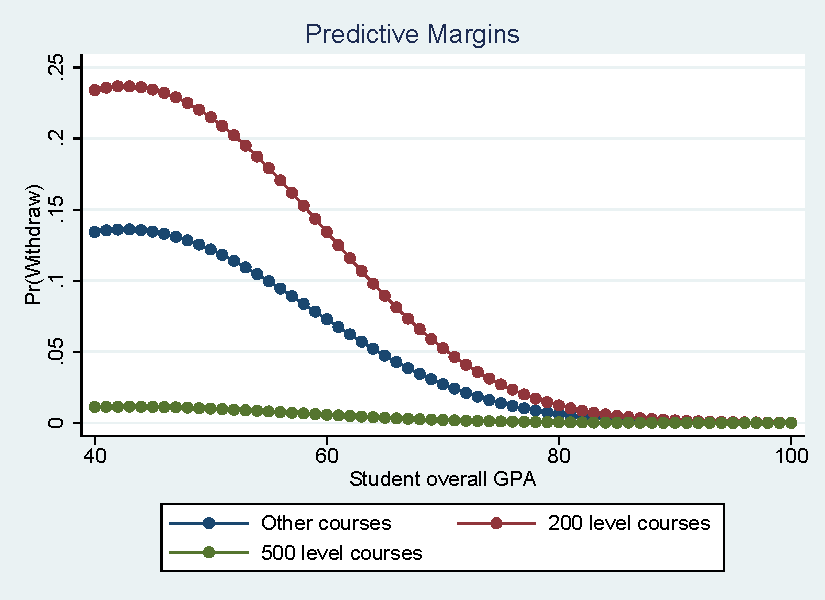
\includegraphics[width=0.7\textwidth]{book_65.pdf}
    \caption{Graphing the probability of withdrawing from a course for different values of GPA for different level courses.}
    \label{fig:visual2}
\end{figure}

The output of this command is shown in Figure ~\ref{fig:visual2}. This graph is interesting because it shows that for 500-level courses, the probability of withdrawal is close to zero no matter what the GPA is. 
The GPA has the largest effect on probability for 200-level courses. This makes sense since at this stage, students will still be uncertain about their choice of major. Getting a low GPA will raise a 
flag that perhaps they are enrolled in the wrong type of course.

A final example will illustrate how we can graph the results when all variables are categorical:

\begin{stlog}. margins, at(gender=(0 1) level3=(0 1 2))
{\smallskip}
Predictive margins                              Number of obs     =     25,160
Model VCE    : OIM
{\smallskip}
Expression   : Pr(withdraw), predict()
{\smallskip}
1._at        : gender          =           0
               level3          =           0
{\smallskip}
2._at        : gender          =           0
               level3          =           1
{\smallskip}
3._at        : gender          =           0
               level3          =           2
{\smallskip}
4._at        : gender          =           1
               level3          =           0
{\smallskip}
5._at        : gender          =           1
               level3          =           1
{\smallskip}
6._at        : gender          =           1
               level3          =           2
{\smallskip}
\HLI{13}{\TOPT}\HLI{64}
             {\VBAR}            Delta-method
             {\VBAR}     Margin   Std. Err.      z    P>|z|     [95\% Conf. Interval]
\HLI{13}{\PLUS}\HLI{64}
         _at {\VBAR}
          1  {\VBAR}   .0102844   .0013374     7.69   0.000     .0076631    .0129057
          2  {\VBAR}   .0199691   .0023579     8.47   0.000     .0153478    .0245904
          3  {\VBAR}   .0007649     .00077     0.99   0.321    -.0007443    .0022741
          4  {\VBAR}   .0156169   .0011701    13.35   0.000     .0133235    .0179103
          5  {\VBAR}    .030048   .0017751    16.93   0.000     .0265689    .0335272
          6  {\VBAR}   .0011728   .0011712     1.00   0.317    -.0011227    .0034683
\HLI{13}{\BOTT}\HLI{64}
{\smallskip}
\end{stlog}

Here, we are calculating the probabilities while varying the variables gender and level3. Note that since GPA was included in the logistic model but was omitted from the margins command, the calculations 
will be done by taking the mean value of GPA. We can visualize the result by using the marginsplot command. The result of running the command is shown in Figure ~\ref{fig:visual3}. We see that the probabilities 
are calculated for females in the three different course levels, as well as for males. We also see that at the 500-level courses, the difference between females and males is minimal, while at the 
200-level courses the difference is considerable.

\begin{stlog}\input{book_67.log.tex}\end{stlog}
\begin{figure}[h]
    \centering
    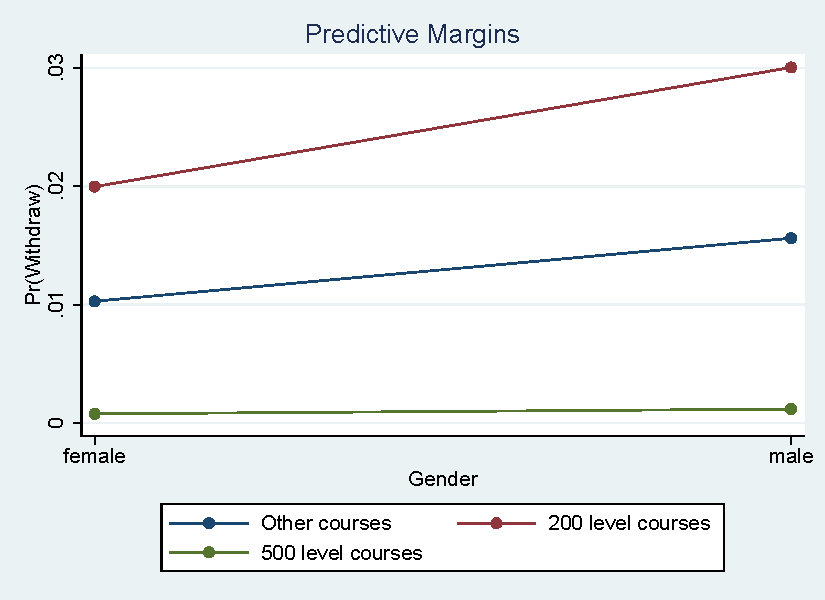
\includegraphics[width=0.7\textwidth]{book_67.pdf}
    \caption{Graphing the probability of withdrawing from a course for different values of gender for different level courses.}
    \label{fig:visual3}
\end{figure}

\chapter{References}
Hilbe, J.M. (2009). Logistic Regression Models. CRC Press.

Hosmer, D.W. \& Lemeshow, S. (2000). Applied Logistic Regression. 2nd edition. Wiley.

Long, J.S. \& Freese, J. (2014). Regression Models for Categorical Dependent Variables using Stata. 3rd ediction. Stata Press.

Mitchell, M.N. (2012). Interpreting and Visualizing Regression Models using Stata. Stata Press.


\end{document}
